
%%%%%%%%%%%%%%%%%%%%%%%% TEMPLATE INFO %%%%%%%%%%%%%%%%%%%%%%%%%%%%%%
%: Template Name = cpe-thesis-th
%: Version Name  = th-vectier-1.1
%: Credits
%: - Peerapon Siripongwutikorn, CPE, 2016
%: - Wuttipat Chokananatasab, FIBO, 2016
%: - Thanin Srithai, CPE, 2021
%: - Jatetanan Kanchanawat, CPE, 2023
%: 
%: This is a LaTeX template used in CPE, KMUTT thesis.
%%%%%%%%%%%%%%%%%%%%%%%%%%%%%%%%%%%%%%%%%%%%%%%%%%%%%%%%%%%%%%%%%%%%%
%: Instructions:
%: Run at the command line:
%: - xelatex <filename> or latexmk -xelatex <filename> to compile
%: tex files
%: - bibtex <filename> or biber <filename> to compile bib file
%: Note: Run a few times to generate the output pdf file
%:
%%%%%%%%%%%%%%%%%%%%%%%%%% REPORT START %%%%%%%%%%%%%%%%%%%%%%%%%%%%%
\documentclass[12pt,one side,openright,a4paper]{cpe-thesis-th}

%%%%%%%%%%%%%%%%%%%%%% Packages and Configs %%%%%%%%%%%%%%%%%%%%%%%%%

\usepackage{color}
\usepackage{pgfgantt}                   % Gantt chart
\usepackage{polyglossia}                % Thai language script and format
\usepackage{caption}                    % Figures and tables captions

\usepackage{etoolbox}                   % Patching commands for macros creating i.e. preto
\usepackage{longtable}                  % Long continuous table
\usepackage{ragged2e}                   % Forcing figure
\usepackage{float}                      % ER and checkmark
\usepackage{tikz}                       % Drawing graphs and symbols
\usepackage{subfig}                     % Subfigures
\usepackage{keyval}                     % Subfigures alignment
\usepackage[export]{adjustbox}          % Subfigures aLignment
\usepackage{cleveref}                   % Clever label references

\usepackage{lmodern}     
\usepackage{listings}                   % Listings as code blocks
\usepackage{packages/listings-golang}   % Listings support for Golang
\usepackage{packages/listings-yaml}     % Listing support for YAML

%: Biblatex for managing bibliography; instead of using old \bibliography{}
%: NOTE: Biblatex define typesetting onto compilation cache.
%: So recompile from scratch (Remove aux and bbl file and recompile)
%: Everytime you stopped using biblatex

% \usepackage[
%     backend=bibtex,     % Biber or Bibtex
%     style=ieee,         % Bib standard
%     sorting=none,       % Sort by appearance in paper
%     % sorting=ynt,       % Sort by year, name...
%     % sortcites=true,    % Some other  example options ...
%     dateabbrev=true,
%     urldate=long,
%     block=none,
%     indexing=false,
%     citereset=none,
%     isbn=true,
%     url=true,
%     language=english,
%     doi=true,           % Prints DOI
%     natbib=true         % if you need Natbib functions
% ]{biblatex} 

%%%%%%%%%%%%%%%%%%% Custom Macros & Settings %%%%%%%%%%%%%%%%%%%%%%%%
%: From this part to \begin{document}
%: Do not modify unless you know what you are doing...

%%%%%%%%%%%%%%%%%%%%%%%%%%%%%%%%%
%%%%%%% Biblatex macro %%%%%%%%%%
%: Uncomment all of these if you're using biblatex

%: Setup URL access date string
% \DefineBibliographyStrings{english}{%
%     urlseen = {accessed}
% }

%: Reference bib files
%: Make sure you reference correct bib file...
% \addbibresource{bib/codern.bib}

%%%%%%%%%%%%%%%%%%%%%%%%%%%%%%%%%
%%%%%%%%%% Typography %%%%%%%%%%%

%: Define 1st and 2nd language
\setdefaultlanguage{thai}
\setotherlanguage{english}

%: Set linebreak to Thai
\XeTeXlinebreaklocale "th"	
\XeTeXlinebreakskip = 0pt plus 0pt
\emergencystretch=10pt

%: Define fonts for code blocks
\newfontfamily\codefont[Scale=0.95]{CourierPrime.ttf}[
    Path=fonts/,
    Extension=.ttf,
    BoldFont=*-Bold,
    ItalicFont=*-Italic,
    BoldItalicFont=*-BoldItalic,
]

%%%%%%%%%%%%%%%%%%%%%%%%%%%%%%%%%
%%%%%% Paragraph Settings %%%%%%%
%: Adjust your paragraph to your standards

\newcommand{\thaijustify}[1]{% 
  \par\hspace{30pt}\justifying
  #1
}

\newcommand{\thaicaption}[1]{% 
  \par\justifying
  #1
}

%%%%%%%%%%%%%%%%%%%%%%%%%%%%%%%%
%%%%%%% Tikz Settings %%%%%%%%%%
%: Tikz is used for drawing simple edge and node graph
%: Import shapes for usage
\usetikzlibrary{er, positioning, shapes.geometric, arrows} 

%: Define checkmark symbol
\def\checkmark{\tikz\fill[scale=0.4](0,.35) -- (.25,0) -- (1,.7) -- (.25,.15) -- cycle;}

%%%%%%%%%%%%%%%%%%%%%%%%%%%%%%%%
%%%%%% Listings Settings %%%%%%%%
%: Listings is used for displaying the program or
%: codes in reports as statement

%: Define text color for code blocks
\definecolor{dkgreen}{rgb}{0,0.6,0}
\definecolor{gray}{rgb}{0.5,0.5,0.5}
\definecolor{mauve}{rgb}{0.58,0,0.82}

%: Go code snippets setting
\lstset{
    frame=tb,
    language=Golang,
    aboveskip=3mm,
    belowskip=3mm,
    showstringspaces=false,
    columns=flexible,
    basicstyle={\small\codefont},
    numbers=left,
    numberstyle=\small\color{gray},
    keywordstyle=\color{blue},
    commentstyle=\color{dkgreen},
    stringstyle=\color{mauve},
    breaklines=false,
    breakatwhitespace=false,
    tabsize=3
}

%%%%%%%%%%%%%%%%%%%%%%%%%%%%%%%%%
%%%%%%%%%% Math macro %%%%%%%%%%%
%: Fraction settings
\renewcommand{\topfraction}{0.85}
\renewcommand{\textfraction}{0.1}

%: Define theorem and proof
\newtheorem{theorem}{Theorem}
\newtheorem{lemma}{Lemma}
\newtheorem{corollary}{Corollary}

\def\QED{\mbox{\rule[0pt]{1.5ex}{1.5ex}}}
\def\proof{\noindent\hspace{2em}{\itshape Proof: }}
\def\endproof{\hspace*{\fill}~\QED\par\endtrivlist\unskip}

%\newenvironment{proof}{{\sc Proof:}}{~\hfill \blacksquare}
%% The hyperref package redefines the \appendix. This one 
%% is from the dissertation.cls
%\def\appendix#1{\iffirstappendix \appendixcover \firstappendixfalse \fi \chapter{#1}}
%\renewcommand{\arraystretch}{0.8}
%%%%%%%%%%%%%%%%%%%%%%%%%%%%%%%%%

%%%%%%%%%%%%%%%%%%%%%% Report Definitions %%%%%%%%%%%%%%%%%%%%%%%%%%%
%: Customize below to suit your needs 
%: The optional ones can be left blank. 

%: Front cover's + signature page's language
%: Enter 'Thai' / 'English' for changing the language 
%: for cover page, appendixes, and signature page
\def\coverlang{Thai}

%: Project Type
%: Enter 'Project' / 'Independent Study' / 'Thesis'
\def\worktype{Project}
\def\thaiworktype{ปริญญานิพนธ์}

%: Credits
%: Enter number based on your subject's credits
\def\disscredit{3}              

%: Fulfillment; 'Degree' or 'Subject'
%: Set to 'Degree' for senior project or thesis
%: 'Subject' for any subject project report i.e. soft-eng final report
\def\fulfillment{Degree}

%: First line of title
\def\disstitleone{Title Line 1}
\def\thaidisstitleone{ชื่อโครงงาน บรรทัด 1}

%: Additional line for title
\def\disstitletwo{Title Line 2}
\def\disstitlethree{Title Line 3}
\def\thaidisstitletwo{ชื่อโครงงาน บรรทัด 2}
\def\thaidisstitlethree{ชื่อโครงงาน บรรทัด 3}

%: Authors
\def\dissauthor{Mr. Krid Hepakrone}  
\def\thaidissauthor{นายกฤษฎิ์ เฮ่ประโคน}
\def\dissauthortwo{Mr. Jatetanan Kanchanawat}
\def\thaidissauthortwo{นายเจตนันท์ กาญจนวัฒน์}
\def\dissauthorthree{Ms. Pimmada Laisuan}
\def\thaidissauthorthree{นางสาวพิมพ์มาดา ไล้สวน}

%: Diploma
%: If you're still an undergraduate having not 
%: graduated from any degree; leave these fields empty
%: Example: B.Eng. (Computer Engineering)
\def\dissdiplomaone{}
\def\dissdiplomatwo{}
\def\dissdiplomathree{}
\def\thaidissdiplomaone{}
\def\thaidissdiplomatwo{}
\def\thaidissdiplomathree{}

%: The degree that you're pursuing..
\def\dissdegree{Bachelor of Engineering} % Name of the degree
\def\thaidissdegree{วิศวกรรมศาสตรบัณฑิต}
\def\dissdegreeabrev{B.Eng.} % Abbreviation of the degree
\def\dissyear{2023}  % Year of submission
\def\thaidissyear{2566} % Year of submission (B.E.)

%: Your project or independent study's committee
%: Example of appropriate advisor/committee name entries
%: Example 1: Asst. Prof. Dr.Ing Priyakorn Pusawiro
%: Example 2: Jaturon Harnsomburana, Ph.D.

%: Advisors
\def\dissadvisor{Assoc. Prof. Natasha Dejdumrong, D. Tech. Sci.} % Advisor
\def\thaidissadvisor{รศ.ดร.ณัฐชา เดชดำรง}

%: Note: Leave empty if you have no co-advisor
\def\disscoadvisor{Asst. Prof Sanan Srakaew} % Co-advisor (optional)
\def\disscoadvisortwo{} % Co-advisor (optional)
\def\thaidisscoadvisor{ผศ.สนั่น สระแก้ว}
\def\thaidisscoadvisortwo{} 

%: Committee
%: Note: Senior projects have no committee chair
\def\disscommitteechair{} % Committee chair (optional)
\def\thaidisscommitteechair{}

%: Note: Leave the following empty if no person is in that position
\def\disscommitteetwo{Asst. Prof. Dr.Ing Priyakorn Pusawiro} % Committee member
\def\disscommitteethree{Asst. Prof. Rajchawit Sarochawikasit} % Committee member (optional)
\def\disscommitteefour{Jaturon Harnsomburana, Ph.D.} % Committee member (optional)
\def\thaidisscommitteetwo{ผศ.ดร.ปริยกร ปุสวิโร}
\def\thaidisscommitteethree{ผศ.ราชวิชช์ สโรชวิกสิต}
\def\thaidisscommitteefour{ดร.จาตุรนต์ หาญสมบูรณ์}

%: Department and Institution Information
\def\institute{King Mongkut's University of Technology Thonburi}
\def\fieldofstudy{Computer Engineering}
\def\department{Computer Engineering} 
\def\faculty{Faculty of Engineering}
\def\thaiinstitute{มหาวิทยาลัยเทคโนโลยีพระจอมเกล้าธนบุรี}
\def\thaifieldofstudy{วิศวกรรมคอมพิวเตอร์} 
\def\thaidepartment{วิศวกรรมคอมพิวเตอร์} 
\def\thaifaculty{วิศวกรรมศาสตร์}

%%%%%%%%%%%%%%%%%%% Front Page / Signature Page %%%%%%%%%%%%%%%%%%%%%
\begin{document}

\pdfstringdefDisableCommands{
\let\MakeUppercase\relax
}

\begin{center}
  
\includegraphics[width=2.8cm]{figure/logo02.jpg}
\end{center}
\vspace*{-1cm}

%: Check fulfillment value
\ifthenelse{\equal{\fulfillment}{Subject}}{
    % Do nothing
}{
    % If not 'Subject', check for 'Degree'
    \ifthenelse{\equal{\fulfillment}{Degree}}{
        % Do nothing
    }{
        % Neither of those, throw error
        \Err{Warning: Invalid fulfillment; use either 'Subject' | 'Degree' (case-sensitive!)}%
        \def\fulfillment{Degree} % Default to Degree
    }
}

%: Check coverlang value and make title page and
\ifthenelse{\equal{\coverlang}{English}}{%
    \maketitlepage%
    \makesignaturepage%
}{%
    \ifthenelse{\equal{\coverlang}{Thai}}{%
        \makethaititlepage%
        \makethaisignaturepage%
    }{%
        \Err{Warning: Invalid coverlang; use either 'English' | 'Thai' (case-sensitive!)}%
        \maketitlepage % Default to English
        \makesignaturepage%
    }%
}%

%%%%%%%%%%%%%%%%%%%%%%%%% English abstract %%%%%%%%%%%%%%%%%%%%%%%%%%

\def\abstcontent{
 \textbf{**ตัวอย่างบทคัดย่อภาษาอังกฤษ}... Proficiency in computer programming is a vital skill in computer science, leading to a surge in student enrollment for programming courses. However, the effectiveness of teaching programming diminishes as class sizes increase, and instructors find it challenging to manually assess each student's assignments promptly. To address this issue, we propose developing a software solution, Coding Platform, a code auto-grading system written in Golang utilizing containerization technology, designed to automate and streamline the grading process. This software aims to evaluate student submissions against predefined test cases, measure resource usage efficiency, and instantly provide feedback and scores. This reduces the burden on instructors and fosters a competitive and engaging learning environment. The platform also maintains a comprehensive record of student performance, aiding both instructors in refining their teaching methods and students in showcasing their achievements. The software had been deployed for its intended use and has, ever since, been tested by both instructors and students alike, in classroom environments and competitive scenes like BangMod Hackathon 2024. Consequently, this grading system has been updated and refined actively as users' bug reports and feature requests are always addressed followed by various updates, fixes, and patches. Overall, the software was very well-received, with survey results averaging an overall score of 8 and good user ratings on the software's functionalities and performance.
}

\def\abstkeyword{
Programming Education / Student Assessment / Golang / Containerization
}

%%%%%%%%%%%%%%%%%%%%%%%%%%% Thai abstract %%%%%%%%%%%%%%%%%%%%%%%%%%%

\def\thabstcontent{
\textbf{**ตัวอย่างบทคัดย่อ...} ความเชี่ยวชาญในการเขียนโปรแกรมคอมพิวเตอร์เป็นทักษะสำคัญในวิทยาการคอมพิวเตอร์ ส่งผลให้ในช่วงมาหลังมีนักศึกษาหันมาสนใจและลงทะเบียนในหลักสูตรการเขียนโปรแกรมเพิ่มมากขึ้น ส่งผลให้ประสิทธิภาพของการสอนการเขียนโปรแกรมจะลดลงเนื่องจากจำนวนผู้เรียนเพิ่มมากขึ้น อาจารย์ผู้สอนพบว่าการประเมินงานมอบหมายของนักเรียนแต่ละคนด้วยตนเองเป็นเรื่องท้าทาย เพื่อแก้ไขปัญหานี้ คณะผู้จัดทำเสนอเเนวทางเเก้ไขปัญหาในรูปเเบบของซอฟต์แวร์ชื่อ Coding Platform ขี้นมาด้วยภาษา Golang และออกแบบด้วยเทคโนโลยี Containerization ระบบซอฟต์แวร์ดังกล่าวจะเป็นระบบสำหรับตรวจโปรแกรมที่นักศึกษาเขียนส่งมาในระบบ แล้วให้ผลตรวจในทันที ซอฟต์แวร์ดังกล่าวจะตรวจและประเมินงานที่ผู้ใช้ส่งมาเทียบกับกรณีทดสอบที่กำหนดไว้ล่วงหน้าและวัดประสิทธิภาพการใช้ทรัพยากรของตัวโปรแกรม จากนั้นจะนำผลตรวจด้งกล่าวไปแสดงในทันที สิ่งนี้ไม่เพียงแต่ช่วยลดภาระของผู้สอนเท่านั้น แพลตฟอร์มดังกล่าวยังรักษาบันทึกผลเเละข้อมููลการใช้งานของผู้ใช้อย่างครอบคลุมเพื่อนำมาเป็นข้อมูลให้อาจารย์ผู้สอนปรับปรุงวิธีการสอนของตน และจัดแสดงความสำเร็จของนักศึกษาเพื่อส่งเสริมสภาพแวดล้อมการเรียนรู้ที่มีการแข่งขันและการมีส่วนร่วม โดยซอฟต์แวร์ดังกล่าวได้ถูกติดตั้งใช้งานแล้ว ซึ่งได้เปิดโอกาสให้ผู้ใช้ทั้งอาจารย์ผู้สอนและนักศึกษาได้ลองใช้งาน ทั้งในห้องเรียนและกิจกรรมวิชาการอย่าง BangMod Hackathon 2024 รวมไปถึงให้ผู้ใช้ได้วิจารณ์และให้คำติชมเพื่อที่จะได้นำไปปรับปรุงและแก้ไขข้อผิดพลาด ซึ่งส่งผลให้ซอฟต์แวร์นั้นได้รับผลตอบรับที่ดีจากผู้ใช้มากมายในแบบประเมินผล ดัวยคะแนนเฉลี่ยของภาพรวมซอฟต์แวร์ที่ 8 คะแนน พร้อมผลคะแนนและคำชมเชยมากมายในด้านความสามารถและประสิทธิภาพการทำงานของซอฟต์แวร์
}

\def\thabstkeyword{
รายวิชาการสอนเขียนโปรแกรม / การวัดและประเมินผลนักศึกษา / ภาษา Golang / เทคโนโลยี Containerization
}

%: Abstract ordered based on cover language
\ifthenelse{\equal{\coverlang}{English}}{%
    \makeabstract%
    \makethaiabstract%
}{%
    \ifthenelse{\equal{\coverlang}{Thai}}{%
        \makethaiabstract%
        \makeabstract%
    }{%
        \Err{Warning: Invalid coverlang; use either 'English' | 'Thai' (case-sensitive!)}%
        \makeabstract%
        \makethaiabstract%
    }%
}%

%%%%%%%%%%%%%%%%%%%%%%%%% Acknowledgments %%%%%%%%%%%%%%%%%%%%%%%%%%%
\preface
\centering{\bf{\textit{(ตัวอย่างกิตติกรรมประกาศ...)}}} \\
\justifying
โครงงานพัฒนาโปรแกรม/แอปพลิเคชัน/เว็บแอปพลิเคชัน สำหรับตรวจงานและข้อสอบในรายวิชาการเรียนการสอนเขียนโปรแกรมภาษาคอมพิวเตอร์ หรือ Coding Platform สามารถบรรลุเป้าหมายไปได้ด้วยดี ทางคณะผู้จัดทำต้องขอขอบคุณผู้สนับสนุนทุกท่านที่ให้การช่วยเหลือในด้านต่าง ๆ ขอขอบคุณ รศ.ดร.ณัฐชา เดชดำรง ที่มาเป็นอาจารย์ที่ปรึกษาโครงการ และสละเวลามาให้ความรู้ พร้อมให้คำแนะนำตลอดการพัฒนาทั้งโครงงาน ขอขอบคุณภาควิชาวิศวกรรมคอมพิวเตอร์ คณะวิศวกรรมศาสตร์ มหาวิทยาลัยเทคโนโลยีพระจอมเกล้าธนบุรี ที่ให้การส่งเสริมและสนับสนุนทางคณะผู้จัดทำ ตลอดจนเอื้อเฟื้อสถานที่และอุปกรณ์สำหรับการพัฒนาโครงงาน ขอขอบคุณนักศึกษาชั้นปีที่หนึ่งและสอง ที่เรียนวิชา CPExxx ..., ... ปีการศึกษาพุทธศักราช 25xx รวมไปถึงนักเรียนชั้นมัธยมศึกษาตอนปลายที่เข้าร่วมโครงการกิจกรรมการเเข่งขันเขียนโปรเเกรมคอมพิวเตอร์ Bangmod Hackathon 20xx ที่จัดขึ้นในปีการศึกษาเดียวกัน ที่สละเวลามาทดลองใช้ซอฟต์เเวร์ต้นแบบ พร้อมทั้งแสดงความเห็น ให้่ข้อเสนอแนะ ให้คำติชมที่ล้วนแต่เป็นข้อมูลอันเป็นประโยชน์ ที่สามารถนำมาใช้ในการพัฒนาซอฟต์แวร์

%%%%%%%%%%%% Table of contents, List of figures/tables %%%%%%%%%%%%%%
%: The three commands below automatically generate the table 
%: of content, list of tables, list of figures, and list of listings

\def\appendixnames{ภาคผนวก} 

\tableofcontents                    
\listoftables
\listoffigures

%%%%%%%%%%%%%%%%%%%%%%%%%% List of codes %%%%%%%%%%%%%%%%%%%%%%%%%%%%
%: Command below automatically will generate the table
%: for listing 'lst' package listings

\listofprograms

%%%%%%%%%%%%%%%%%%%%%%%%%% List of symbols %%%%%%%%%%%%%%%%%%%%%%%%%%
%: You have to add this manually...

\listofsymbols
\justifying{
    \centering{\bf{\textit{(ตัวอย่างสารบัญสัญลักษณ์...)}}} \\
    %: You can adjust width to suit your word length
    \begin{tabular}{@{}p{0.07\textwidth}p{0.7\textwidth}p{0.1\textwidth}}
        \textbf{สัญลักษณ์} & & \textbf{หน่วย} \\[0.2cm]
            $\alpha$ & Test variable\hfill & m$^2$ \\
            $\lambda$ & Interarival rate\hfill &  jobs/second\\
            $\mu$ & Service rate\hfill & jobs/second\\
    \end{tabular}
}

%%%%%%%%%%%%%%%%%%%%% List of vocabs & terms %%%%%%%%%%%%%%%%%%%%%%%%
%: You also have to add this manually...

\newcommand{\tableraglf}[1]{\RaggedRight{#1}}
\listofvocab
\begin{flushleft}
    \centering{\bf{\textit{(ตัวอย่างสารบัญคำศัพท์...)}}} \\
    %: You can adjust width to suit your word length
    \begin{tabular}{@{}p{1.2in}@{\hspace{0.08in}=\extracolsep{0.2in}}p{4in}}
        PDF & \tableraglf{ย่อมาจาก Portable Document File แปลว่ารูปแบบไฟล์เอกสารที่สามารถเคลื่อนย้ายไปมาได้อย่างสะดวก} \\
        UI / ส่วนประสานงานผู้ใช้ & \tableraglf{ย่อมาจาก User Interface ในภาษาอังกฤษ หมายถึงส่วนที่ให้ผู้ใช้งานสามารถโต้ตอบกับการใช้งานผลิตภัณฑ์ได้ ซึ่งจะมุ่งเน้นไปที่เรื่องของหน้าตา การออกแบบ เช่น หน้าจอ แพลตฟอร์ม เมนู ฟอร์ม}  \\ 
        UX / ประสบการณ์ของผู้ใช้ &  \tableraglf{ย่อมาจาก User Experience ในภาษาอังกฤษ ประสบการณ์ของผู้ใช้งานในด้านความรู้สึกที่ตอบสนองต่อการใช้งานผลิตภัณฑ์ หรือระบบต่าง ๆ ยกตัวอย่างเช่น ความสะดวกสบาย ใช้งานง่าย ความสนุกสนาน}  \\
        MD & \tableraglf{ย่อมาจากคำว่า Markdown ซึ่งเป็นภาษา Markup ที่เรียบง่าย ที่มีความคล้ายคลึงกับภาษามนุษย์ โดยหลักการเขียนอิงตามแบบแผนข้อความธรรมดา (plain text) ที่ผ่านการทดสอบและรวบรวมเป็นมาตรฐาน อิงจากข้อมูลที่เก็บเป็นช่วงเวลา 40 ปีที่ผ่านมา} \\
    \end{tabular} 
\end{flushleft}

%\setlength{\parskip}{1.2mm}

%%%%%%%%%%%%%%%%%%%%%%%%% Introduction %%%%%%%%%%%%%%%%%%%%%%%%%%%%%%

\chapter{บทนำ}
\section{ที่มาและความสำคัญ}
    \centering{\bf{\textit{(ตัวอย่างปัญหา...)}}} \\
    \thaijustify{
        ทักษะการเขียนโปรแกรมคอมพิวเตอร์เป็นทักษะที่สำคัญสำหรับวิชาชีพในสาขาวิทยาการคอมพิวเตอร์ เป็นเหตุให้นักศึกษาจำนวนมากหันมาสมัครหรือลงวิชาเขียนโปรแกรมคอมพิวเตอร์เพิ่มมากขึ้น ทำให้การเรียนการสอนวิชาเขียนโปรแกรมคอมพิวเตอร์มีประสิทธิภาพที่ต่ำลงเพราะจำนวนผู้เรียนมากขึ้น อาจารย์ผู้สอนไม่สามารถจะดูแลนักศึกษาได้ครบทุกคน การตรวจงานและให้คะแนนใช้ระยะเวลานาน เพราะอาจารย์ผู้สอนจะต้องนำไฟล์งานของนักศึกษามาตรวจทีละไฟล์ อีกทั้งยังมีโอกาสเกิดข้อผิดพลาดในการตรวจอีกด้วย
    }
    \thaijustify{
        จากปัญหาดังกล่าว...
    }
    \thaijustify{
        โดยซอฟต์แวร์จะ...
    }
\section{วัตถุประสงค์}
    ทางกลุ่มเรา ได้ดำเนินโครงการพัฒนาซอฟต์เเวร์ดังกล่าว ด้วยวัตถุประสงค์ดังต่อไปนี้
    \begin{enumerate}
        \item เพื่อ...
        \item เพื่อ...
        \item เพื่อ...
    \end{enumerate}

\section{ขอบเขตของโครงงาน}
    \begin{enumerate}
        \item ซอฟต์แวร์รองรับการแสดงผลเป็นภาษาอังกฤษและภาษาไทย...
        \item ซอฟต์แวร์เน้นการใช้งานบนหน้าจอมือถือ...
        \item มีระบบ...
        \item ระบบรองรับ
        \begin{enumerate}
            \item เงื่อนไข...
            \item สามารถ...
        \end{enumerate}
    \end{enumerate}

%: NOTE: This should not be included in thesis, but in proposals
\section{ประโยชน์ที่คาดว่าจะได้่รับ}
    หลังจากสิ้นสุดโครงการ ทางคณะผู้จัดทำคาดหวังว่า โครงการดังกล่าวจะให้ผลประโยชน์ต่อทั้งตนเเละผู้อื่น ดังต่อไปนี้
    \begin{enumerate}
        \item ทางคณะผู้จัดทำจะได้รับ...
        \item อาจารย์ได้...
        \item ทางภาควิชาได้....
    \end{enumerate}

\pagebreak
\section{ตารางการดำเนินงาน}
    \centering{\bf{\textit{(ตัวอย่าง Gantt Chart...)}}} \\
    \thaijustify{
        ในส่วนนี้เป็นแผนและตารางเวลาของแต่ละขั้นตอน...
    }
\begin{table}[!h]
    \centering
    \caption{ตารางการดำเนินการในภาคการศึกษาที่ 1}
    \label{tbl:gantt1}
    \begin{ganttchart}[
        x unit = 0.5cm,
        y unit chart = 1.2cm,
        y unit title = 0.6cm,
        title height = 1,
        vgrid={*{3}{black, dotted}, *1{black, dashed}},
        hgrid={*1{black, dashed}},
        bar top shift = 0.1, 
        %bar height = 0.8,
        bar label node/.append style={
            align=right,
            text width=width("7. จัดทำรายงานของภาคการศึกษาที่ 1")
        }
    ]{1}{20}
        \gantttitle{สิงหาคม}{4} \gantttitle{กันยายน}{4} \gantttitle{ตุลาคม}{4} \gantttitle{พฤศจิกายน}{4} \gantttitle{ธันวาคม}{4} \\
        \gantttitlelist{1,...,4}{1} \gantttitlelist{1,...,4}{1} \gantttitlelist{1,...,4}{1} \gantttitlelist{1,...,4}{1} \gantttitlelist{1,...,4}{1} \\
        \ganttbar{ศึกษาค้นคว้า วิเคราะห์หาปัญหาและที่มา}{2}{2} \\
        \ganttbar{เสนอหัวข้อโครงงาน}{3}{3} \\
        \ganttbar{ศึกษาค้นคว้า หาข้อมูลที่เกี่ยวข้อง}{3}{4} \\
        \ganttbar{นำเสนอโครงการให้กับอาจารย์ที่ปรึกษา}{4}{4} \\
        \ganttbar{จัดทำข้อเสนอโครงการ}{5}{9} \\
        \ganttbar{นำเสนอข้อเสนอโครงการ}{11}{11} \\
    \end{ganttchart}
\end{table}

\begin{table}[!h]
    \centering
    \caption{ตารางการดำเนินการในภาคการศึกษาที่ 2}\label{tbl:gantt2}
    \begin{ganttchart}[
       x unit = 0.5cm,
        y unit chart = 1.2cm,
        y unit title = 0.6cm,
        title height = 1,
        vgrid={*{3}{black, dotted}, *1{black, dashed}},
        hgrid={*1{black, dashed}},
        bar top shift = 0.1, 
        %bar height = 0.8,
        bar label node/.append style={
            align=right,
            text width=width("7. จัดทำรายงานของภาคการศึกษาที่ 1")}
]   {1}{20}
        \gantttitle{มกราคม}{4} \gantttitle{กุมภาพันธ์}{4} \gantttitle{มีนาคม}{4} \gantttitle{เมษายน}{4} \gantttitle{พฤษภาคม}{4} \\
        \gantttitlelist{1,...,4}{1} \gantttitlelist{1,...,4}{1} \gantttitlelist{1,...,4}{1} \gantttitlelist{1,...,4}{1} \gantttitlelist{1,...,4}{1} \\
        \ganttbar{พัฒนาซอฟต์แวร์และระบบ (ต่อจากภาคการศึกษาที่ 1)}{1}{1} \\
    \end{ganttchart}
\end{table}
\pagebreak

%%%%%%%%%%%%%%%%%%%%%%%% Literature Review %%%%%%%%%%%%%%%%%%%%%%%%%%

\chapter{ทฤษฎีความรู้และงานที่เกี่ยวข้อง}
\centering{\bf{\textit{(ตัวอย่างเนื้อหาบทที่สอง...)}}} \\
\thaijustify{
    ในบทที่ 2 จะ...
}
\section{ทฤษฎีที่เกี่ยวข้อง}
    \thaijustify{
        ในโครงงานพัฒนาซอฟต์แวร์นี้ ทางกลุ่มได้ทำการศึกษาค้นคว้า...
    }
    \subsection{ทฤษฎีการเขียนโปรแกรมแบบเชิงวัตถุ}
        \thaijustify{
            ทฤษฎีการเขียนโปรแกรมเชิงวัตถุ (Object-Oriented Programming Theory) เป็นแนวคิดในการออกแบบและพัฒนาซอฟต์แวร์ที่เน้นการแบ่งงานออกเป็นองค์ประกอบที่มีลักษณะคล้ายกับวัตถุจริง ๆ ในโลกทั่วไป ถ้าอิงจากวัตถุในชีวิตจริงก็แสดงว่า วัตถุนั้นมีสถานะ (State), พฤติกรรม (Behavior) และความสัมพันธ์ (Relationship) ระหว่างกัน~\cite{booch87} ในการใช้ทฤษฎีเชิงวัตถุในการพัฒนาซอฟต์แวร์ เราสามารถสร้างองค์ประกอบหรือวัตถุที่มีความสมบูรณ์และเป็นรูปแบบสำหรับแก้ปัญหาแต่ละประเภทได้อย่างมีประสิทธิภาพ~\cite{meyer2000}
        }
        \thaijustify{
            การใช้ทฤษฎีเชิงวัตถุมีข้อได้เปรียบหลายประการ เช่นช่วยลดความซับซ้อนของโค้ดหรือทำให้การบำรุงรักษาซอฟต์แวร์ง่ายขึ้น (Maintainability) เพิ่มความยืดหยุ่นในการพัฒนา (Extendability) และเปิดโอกาสในการนำวัตถุที่มีอยู่แล้วในซอฟต์แวร์มาใช้งานใหม่ (Reusability) การแบ่งงานเป็นวัตถุ (หรือ Object) ย่อย ๆ ทำให้โค้ดมีโครงสร้างที่เรียบง่ายและเป็นระเบียบ เพราะฉะนั้นทำให้การทำงานของโปรแกรมเป็นไปอย่างมีประสิทธิภาพและมั่นคง~\cite{meyer2000}
        }
        \begin{figure}[H]
            \centering
            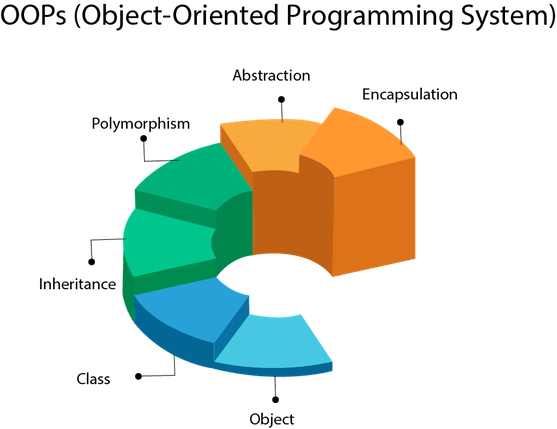
\includegraphics[width=7cm]{figure/literature/oop-programming.png}
            \caption[แผนผังองค์ประกอบของ OOPs]{แผนผังองค์ประกอบของการเขียนโปรแกรมแบบเชิงวัตถุ จาก~\cite{apollo22oop}}
            \label{fig:oop-concept}
        \end{figure}
        \thaijustify{
            องค์ประกอบของระบบโปรแกรมแบบเชิงวัตถุ (\cref{fig:oop-concept}) หรือ Object-Oriented Program System (หรือเรียกโดยย่อว่า OOPs) มีองค์ประกอบดังต่อไปนี้ 
        }
        \subsubsection{การทำ Encapsulation}
            \thaijustify{
                Encapsulation เป็นเหมือนการรวมข้อมูลและฟังก์ชันเข้าด้วยกัน จากงานศึกษาค้นคว้าของ \textit{Nzerue-Kenneth et al.}~\cite{nzeruekenneth23polymorph} เหมือนกับการใส่ไว้ในแคปซูลป้องกัน แนวคิดหลักคือการซ่อนความซับซ้อนของ Objects จากโปรแกรมและผู้ใช้ ทำให้ใช้งานได้ง่ายขึ้น มันคือทั้งหมดที่เกี่ยวกับการซ่อนการทำงานภายในของโค้ดไว้ ดังนั้นจึงไม่ต้องกังวลเกี่ยวกับวิธีการทำงาน แค่ใช้งานอย่างเดียวเท่านั้น
            }
            \begin{figure}[H]
                \centering
                \subfloat[การเปรียบเทียบการทำ Encapsulation กับยาแคปซูล~\cite{raut22encapsule}]{
                    \fbox{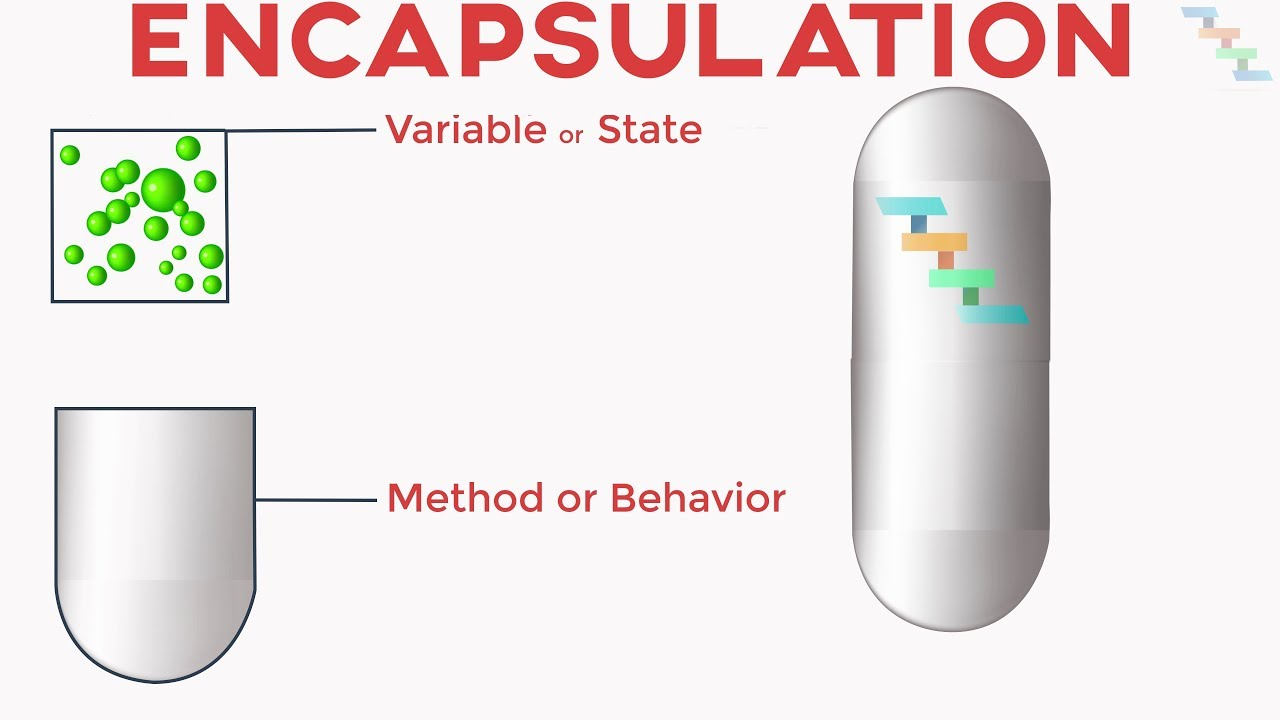
\includegraphics[width=6cm]{figure/literature/oop-encapsulation.png}}
                    \label{fig:oop-encapsulation-capsule}
                }
                \subfloat[การทำ Encapsulation เพื่อปกปิดคุณสมบัติของคลาส~\cite{nishad22encapsulation}]{
                    \fbox{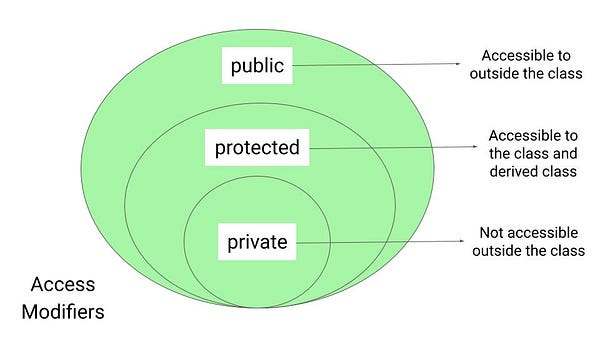
\includegraphics[width=6cm]{figure/literature/oop-encapsulation-detail.jpg}}
                    \label{fig:oop-encapsulation-details}
                } 
                \caption[แผนผังอธิบายการทำ Encapsulation]{แผนผังอธิบายการทำ Encapsulation}
                \label{fig:oop-encapsulation}
            \end{figure}
            \thaijustify{
                จากบทความของ \textit{Raut A.}~\cite{raut22encapsule} ได้เปรียบเทียบหลักการนี้กับแคปซูลที่ปกป้องยาที่อยู่ภายใน ตามในรูปที่~\ref{fig:oop-encapsulation-capsule} การห่อหุ้มของแคปซูลจะปกป้องข้อมูลและฟังก์ชันในโปรแกรม มันเชื่อมโยงโค้ดและข้อมูลที่มันทำงานด้วย สร้างเกราะป้องกันล้อมรอบพวกมัน ด้วยการห่อหุ้ม คุณสามารถจำกัดการเข้าถึงบางส่วนของออบเจ็กต์ โดยให้เฉพาะส่วนอื่น ๆ ของโปรแกรมเข้าถึงสิ่งที่พวกเขาต้องการเท่านั้น เหมือนกับมีตู้จำหน่ายสินค้าอัตโนมัติ คุณไม่สามารถเข้าไปซื้อขนมข้างในได้เว้นแต่คุณจะใช้ปุ่มของเครื่อง ในทำนองเดียวกัน ในการห่อหุ้ม ตัวแปรและฟังก์ชันของวัตถุจะถูกซ่อนไว้และสามารถเข้าถึงได้ผ่านวิธีการเฉพาะภายในคลาสของวัตถุนั้นเท่านั้น
            }
            \thaijustify{
                ดังนั้น การทำ Encapsulation คือทั้งหมดที่เกี่ยวกับการเก็บรักษาสิ่งของต่างๆ ให้ปลอดภัยและซ่อนไว้ตามรูปที่~\ref{fig:oop-encapsulation-details} เช่นเดียวกับยาในแคปซูลหรือของว่างในตู้จำหน่ายสินค้าอัตโนมัติ ช่วยให้โปรแกรมใช้งานและเข้าใจได้ง่ายขึ้นโดยปกป้องการทำงานภายในของโปรแกรมเหล่านั้น~\cite{nishad22encapsulation}
            }
\section{โครงงาน งานวิจัยหรือผลิตภัณฑ์ที่เกี่ยวข้อง}
    เนื่องจาก... กลุ่มเราจึงศึกษา... มาใช้อ้างอิง... นำมาประยุกต์ใช้ใน...
    \subsection{IPST Program Grader}
        \thaijustify{
            \href{https://programming.in.th}{IPST Program Grader} เป็นเว็บไซต์ แอปพลิเคชันที่สร้างขึ้นโดย\textit{สถาบันส่งเสริมการสอนวิทยาศาสตร์และเทคโนโลยี (สสวท.)}~\cite{ipstGrader} ถูกนำมาปรับปรุงใหม่โดยกลุ่มนักเรียนค่ายโอลิมปิกวิชาการคอมพิวเตอร์ในช่วงล่าสุดนี้ เว็บไซต์ดังกล่าวถูกสร้างขึ้นมาเพื่อให้ผู้ใช้สามารถเข้ามาฝึกฝนทักษะการเขียนโปรแกรม เรียนรู้การเขียนโปรแกรม เรียนรู้เกี่ยวกับโครงสร้างข้อมูล และฝึกเขียนอัลกอริทึมที่มีประสิทธิภาพ
        }
        \begin{figure}[H]
            \centering
            \subfloat[หน้าหลักเว็บไซต์ ณ วันที่ 10 ธันวาคม 2562~\cite{ipstGrader}]{
                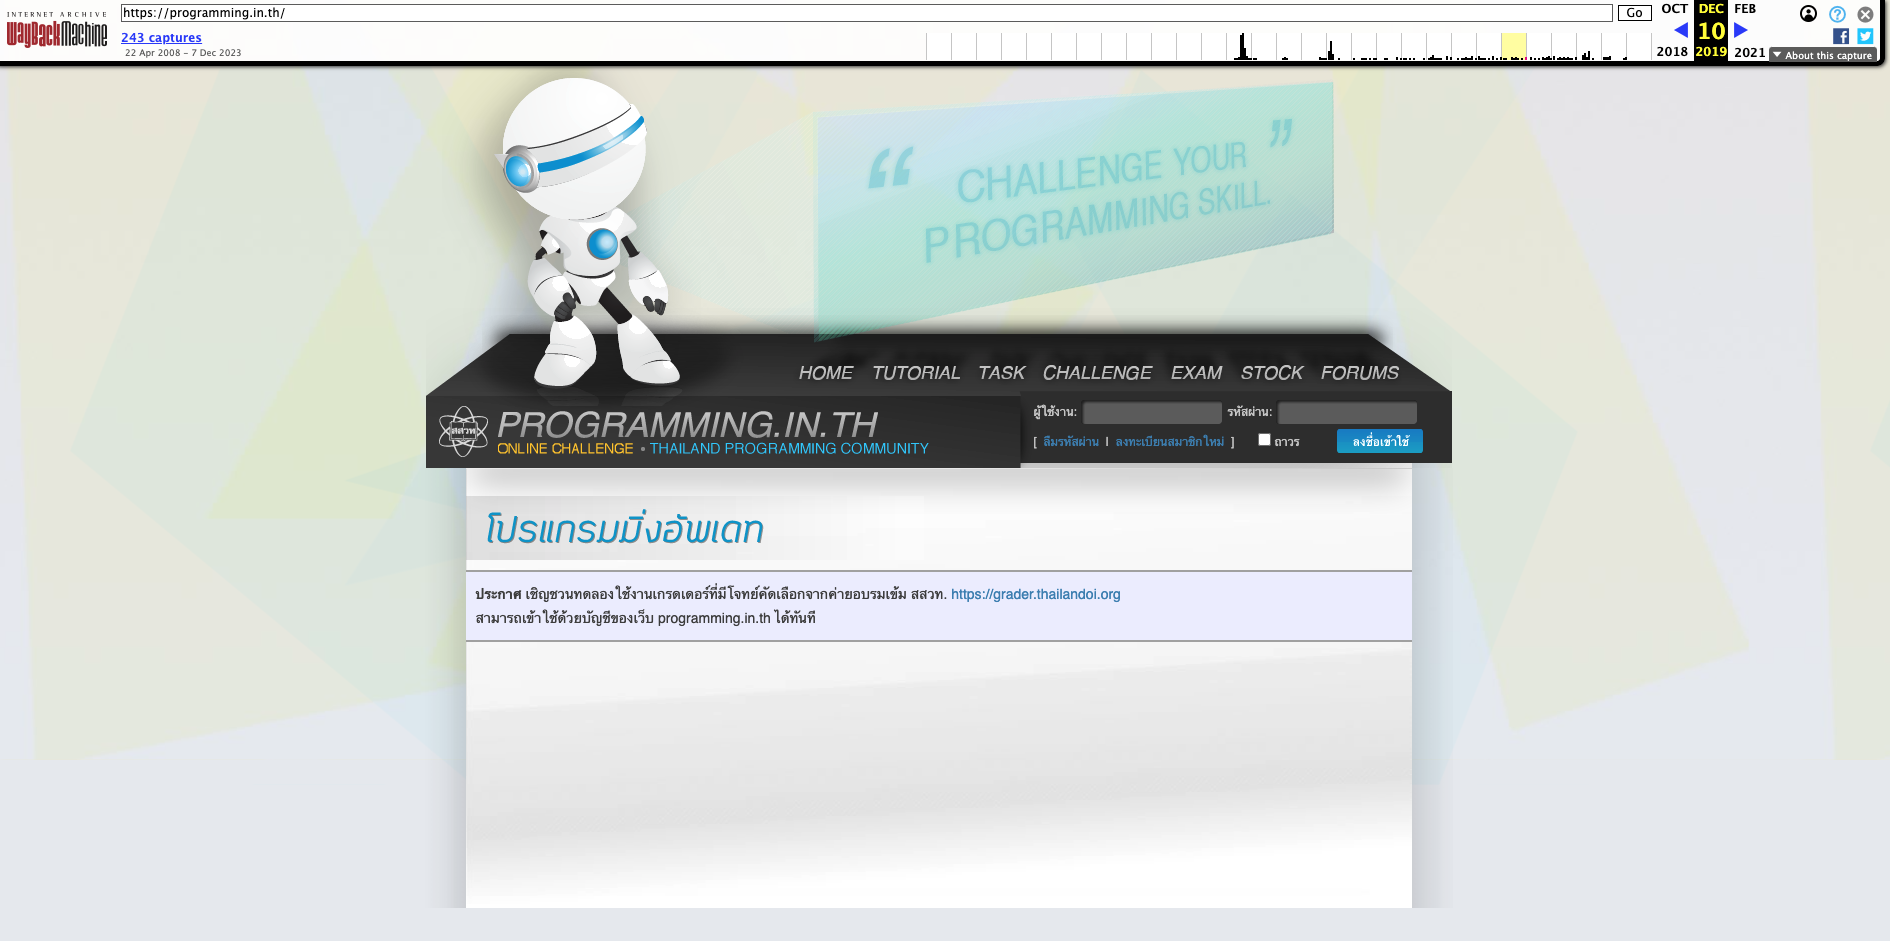
\includegraphics[width=7cm]{figure/literature/old-ipst.png}
                \label{fig:ipst-page-old}
            }
            \subfloat[หน้าหลักเว็บไซต์ ณ ปัจจุบัน]{
                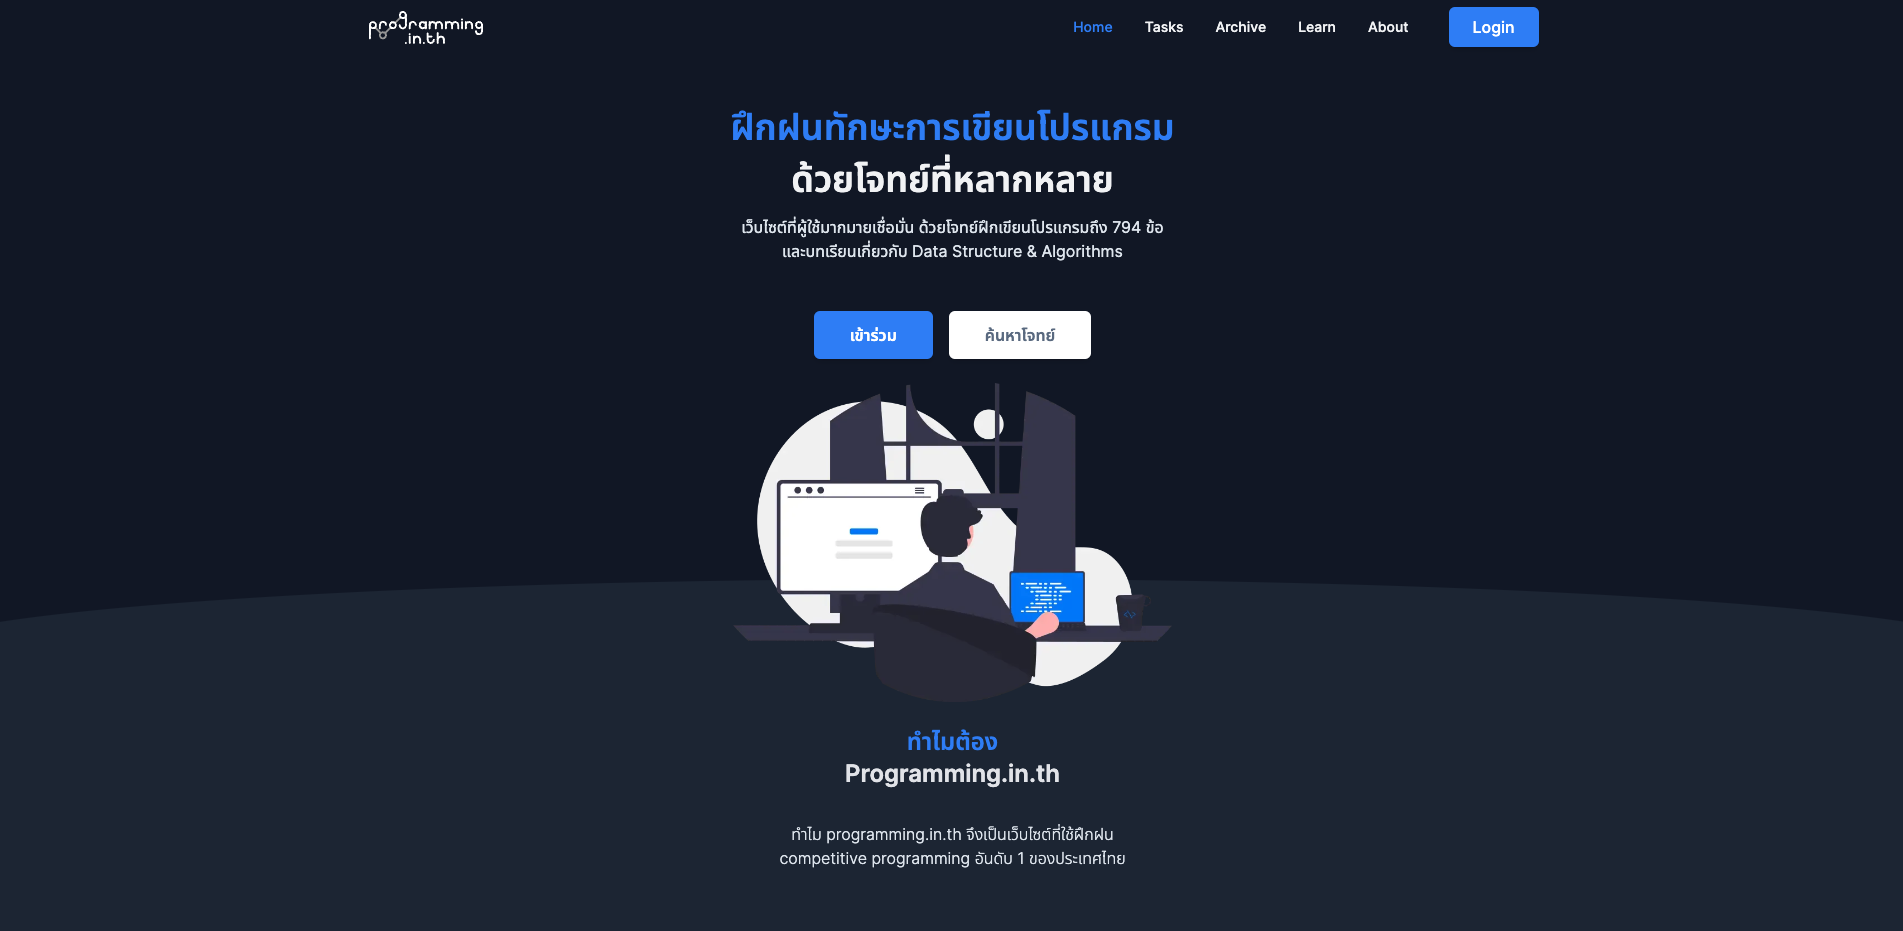
\includegraphics[width=7cm]{figure/literature/current-ipst.png}
                \label{fig:ipst-page-new}
            } 
            \caption[หน้าหลักของ IPST Program Grader]{หน้าหลักของ IPST Program Grader}
            \label{fig:ipst-page}
        \end{figure}
        \thaijustify{
            เว็บไซต์นี้มีฐานข้อมูลโจทย์ปัญหาที่แต่งโดยทางสสวท. ที่ผู้ใช้สามารถกดเลือกเข้าไปทำข้อไหนก็ได้ มีระบบสมัครสมาชิก และมีแหล่งเรียนรู้เพิ่มเติม (Learning resource) สำหรับให้ผู้ใช้ได้เข้าอ่านทำความเข้าใจและเรียนรู้การเขียนโปรแกรม
        }
        \thaijustify{
            เว็บไซต์ดังกล่าวเป็นหนึ่งในแรงบันดาลใจ ต้นฉบับความคิดและต้นแบบซอฟต์แวร์ที่~\cite{nattawat20pgs} ใช้เป็นตัวอย่างในเชิงของแนวคิดในการออกแบบซอฟต์แวร์
        }
        \thaijustify{
                ใน \textit{Jamlongrad et al.}~\cite{nattawat20pgs} ได้มีการวิเคราะห์ สรุปข้อดีและข้อเสียของระบบ แต่เนื่องจากเว็บไซต์ได้มีการเปลี่ยนแปลงในรอบปีที่ผ่านมา คณะผู้จัดทำก็ได้ไปสำรวจการทำงานเว็บไซต์ใหม่อีกรอบหนึ่ง แล้วนำผลสำรวจมาสรุปรวบยอดกับในรายงานดังกล่าว สรุปเป็นผลเป็น~\cref{tbl:ipst-pro-cons} ดังต่อไปนี้
        }
        \begin{table}[H]
            \centering
            \caption{ข้อดีและข้อเสียของระบบ IPST Grader}
            \label{tbl:ipst-pro-cons}
                \begin{tabular}{p{1cm}|p{6cm}|p{6cm}} \hline\hline
                    ข้อที่ & ข้อดี & ข้อเสีย \\ 
                    \hline\hline
                    1. & \RaggedRight{เว็บไซต์มีระบบการตรวจและประเมินผลโปรแกรมที่รวดเร็ว ผู้ใช้สามารถรับรู้ผลได้ทันที}\par & \RaggedRight{เว็บไซต์ไม่สามารถจะใช้งานเครือข่ายเฉพาะได้ เพราะเว็บไซต์ดังกล่าวอยู่ในเครือข่ายสาธารณะ ทำให้เว็บไซต์นี้ไม่สามารถนำมาใช้ในการแข่งขันภายในได้}\par \\ \hline
                    2. & \RaggedRight{ส่วนประสานผู้ใช้ถูกออกแบบมาอย่างดี เพื่อความสะดวกสบายของผู้ใช้}\par & \RaggedRight{ไม่มีระบบสื่อสาร ไม่มีระบบกระทู้สนทนา ไม่มีช่องทางการสื่อสารให้ผู้ใช้ได้คุยปรึกษากันเรื่องโจทย์}\par \\ \hline
                    3. & \RaggedRight{เว็บไซต์มีโจทย์ปัญหาที่หลากหลาย แต่งแต่ระดับง่ายสุด ไปยังระดับการแข่งขันระดับนานาชาติ}\par & \RaggedRight{ผู้ใช้ไม่สามารถเพิ่มโจทย์ปัญหาเองได้ โจทย์ปัญหาถูกควบคุมและเพิ่มโดยผู้ดูแลเว็บเท่านั้น}\par \\ \hline
                    4. & \RaggedRight{เว็บไซต์มีระบบจัดหมวดหมู่โจทย์ปัญหา ทำให้ผู้ใช้หาโจทย์ปัญหาที่ต้องการทำได้ง่าย}\par & \\
                    \hline\hline
                \end{tabular}   
        \end{table}

\section{ภาษาคอมพิวเตอร์เเละเทคโนโลยี}
    \thaijustify{
        หลังจาก... ทางกลุ่มจะอธิบาย... เครื่องมือ เทคโนโลยีและซอฟต์แวร์...
    }
    \subsection{ภาษาคอมพิวเตอร์}
        \thaijustify{
            เพราะ... ทางกลุ่มจึงได้ไปศึกษาหาภาษาคอมพิวเตอร์...
        }
        \subsubsection{ภาษา Go}
            \thaijustify{
                ภาษา Go หรือที่รู้จักกันอย่างแพร่หลายว่า Golang เป็นภาษาโปรแกรมเปิดต้นทางที่พัฒนาโดยทีมนักพัฒนาซอฟต์แวร์ที่ Google โดยรวมถึง Robert Griesemer, Rob Pike, และ Ken Thompson เหล่านักพัฒนาที่ในไม่กี่ทศวรรษก่อน พัฒนาภาษา C ขึ้นมา ภาษา Go นั้นถูกออกแบบขึ้น เพื่อแก้ไขข้อจำกัดของภาษาโปรแกรมเดิมที่มีอยู่แล้วทั้งในด้านประสิทธิภาพ (Efficiency) ความเรียบง่าย (Simplicity) และการสนับสนุนการทำงานพร้อมกัน (Concurrency มีไวยากรณ์ (Syntax) ที่กระชับ การกำหนดประเภท (Type) ที่แข็งแรง พร้อมทั้งระบบจัดการทรัพยากรขยะของโปรแกรม (Garbage Collection) ที่มีประสิทธิภาพ~\cite{pike12go, donovan15go}
            }
            \thaijustify{
                จากความเห็นของ \textit{Pike R.} ใน~\cite{pike12go, pike12godev} หนึ่งในลักษณะที่ดีเด่น Go คือการให้ความสำคัญกับความเรียบง่ายและความอ่านง่าย ทำให้เป็นทางเลือกที่ยอดเยี่ยมสำหรับทั้งผู้เริ่มต้นและนักพัฒนาที่มีประสบการณ์มาก มันนำเสนอแนวทางที่มีความเรียบง่าย ป้องกันความซับซ้อนที่ไม่จำเป็น และมีไวยากรณ์ที่ถูกต้องและโดดเด่น ภาษานี้รวมถึงคุณสมบัติที่สนับสนุนการทำงานพร้อมกันที่ซึ่งช่วยให้นักพัฒนาสามารถเขียนแอปพลิเคชันที่มีประสิทธิภาพและมีขนาดใหญ่ได้
            }
            \thaijustify{
                การทำงานพร้อมกันหรือ Concurrency ก็เป็นแข็งสำคัญของ Go อย่างหนึ่ง การทำ Concurrency ในภาษา ทำผ่าน Channel และ GoRoutines ซึ่งเป็น Thread ที่ Light-weighted ทำให้สามารถสร้างโปรแกรมที่ทำงานพร้อมกันได้โดยไม่มีความซับซ้อน~\cite{donovan15go}
            }
            \thaijustify{
                เนื่องจาก ภาษา Go นั้นกำลังได้รับความนิยมในหลาย ๆ ด้าน ณ ปีการศึกษานี้เช่น การสร้างหรือพัฒนาเว็บไซต์ เว็บแอปพลิเคชัน, การสร้างระบบบริการ Cloud, การสร้างซอฟต์แวร์ระบบที่มีประสิทธิภาพ เป็นต้น ภาษา Go เป็นภาษาที่ใช้งานง่าน และสามารถรันโปรแกรมที่อาศัยการทำงานหรือประมวลแบบ Parallel และ Concurrent~\cite{golangorg} ด้วยเหตุนี้บริษัทใหญ่หลายบริษัทในยุคใหม่ที่มีระบบซอฟต์แวร์ที่ใหญ่ จึงนิยมใช้ภาษาดังกล่าว แล้วเนื่องด้วยสมาชิกในกลุ่มคณะผู้จัดทำได้มีโอกาสไปฝึกงานบริษัทที่ใช้ภาษาดังกล่าว จึงเห็นเป็นโอกาสนำความรู้และความเข้าใจมาประยุกต์ในโครงงานนี้
            }
    \subsection{เครื่องมือและซอฟต์แวร์โครงสร้างพื้นฐาน}
        เพราะ... กลุ่มเราจึงได้มีการค้นคว้า...
        \subsubsection{เว็บเฟรมเวิร์ค React}
            \thaijustify{
                React เป็นไลบรารี JavaScript ที่ถูกพัฒนาขึ้นโดย Facebook สำหรับสร้าง User Interface (UI) ที่ได้รับความนิยมอย่างแพร่หลายในการพัฒนาเว็บแอปพลิเคชัน (web applications)~\cite{flanagan20js}
            }
            \begin{figure}[H]
                \centering
                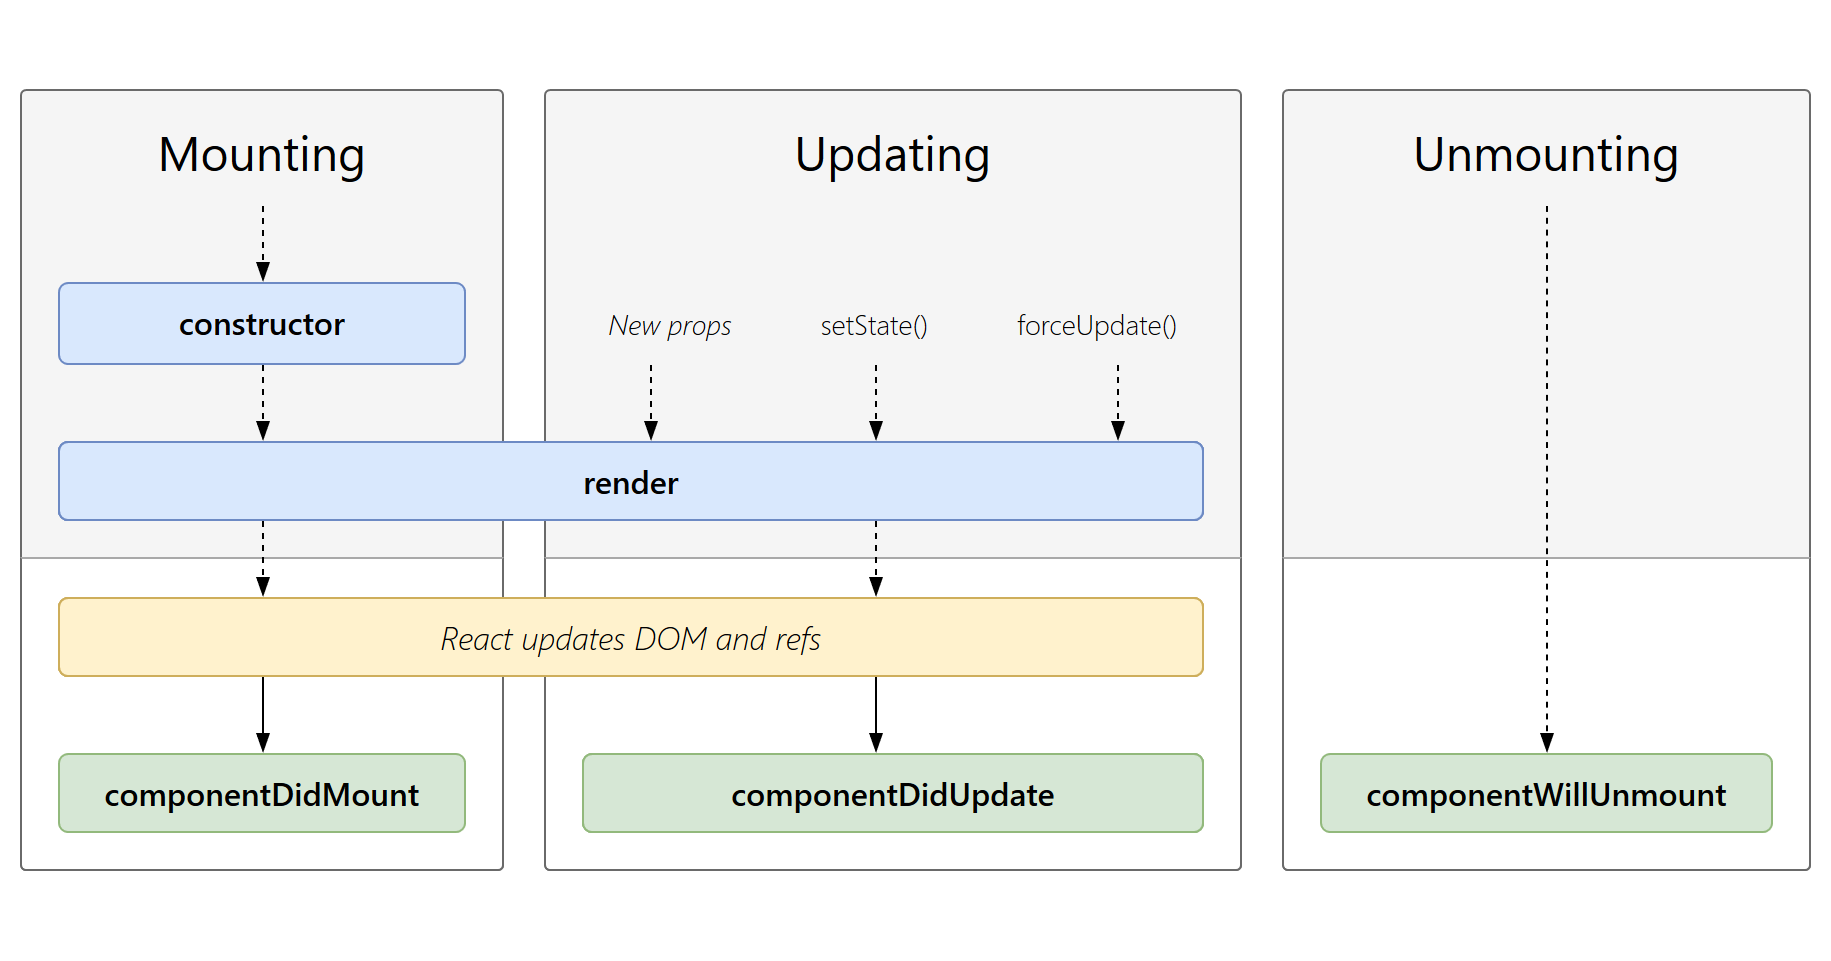
\includegraphics[width=12cm]{figure/literature/react-lifecycle.png}
                \caption[วัฏจักรการทำงานของ React]{วัฎจักรการ Render, Mount-Unmount และ Update ของ React (React Lifecycle) จาก~\cite{reactcycles}}\label{fig:lit-react}
            \end{figure}
            \thaijustify{
                React ให้เครื่องมือและโครงสร้างที่สำหรับการสร้างชิ้นส่วนประกอบของส่วนประสานงานผู้ใช้หรือ UI components ได้หลากหลายและมีประสิทธิภาพ~\cite{crockford08js} หนึ่งในข้อได้เปรียบของ React อยู่ที่การใช้ Virtual DOM ที่ช่วยเพิ่มประสิทธิภาพของการ Render องค์ประกอบของ UI และการสร้างแอปพลิเคชันที่มีประสิทธิภาพและสามารถบริหารจัดการ State ของแอปพลิเคชันได้ง่าย~\cite{flanagan20js}...
            }
\section{สรุปการศึกษาค้นคว้า}
    \thaijustify{
        จาก... คณะผู้จัดทำได้นำหลักการ วิทยาการ และเทคโนโลยี นำไปประยุกต์...
    }
    \subsection{การประยุกต์ใช้ทฤษฎีและหลักการ}
        \thaijustify{
            หลักการเขียนโปรแกรมเชิงวัตถุหรือ OOPs จาก~\cite{booch87, meyer2000, apollo22oop} เป็นหลักการเขียนโปรแกรมที่มีประโยชน์อย่างมาก สามารถที่จะทำให้ผู้พัฒนาซอฟต์สามารถที่จะออกแบบและสร้างที่มีความต้องการและมีการทำงานขึ้นมาได้อย่างง่ายได้ หากใช้ร่วมกับแนวคิดการออกแบบแยกข้อกังวลและแยกความรับผิดชอบหรือ SoC นั้น จะทำให้ระบบซอฟต์แวร์มีส่วนการทำงานที่ถูกนิยามและวางไว้อย่างชัดเจน มีหน้าถ้าหากส่วนใดเกิดปัญหาขึ้นมาในส่วนใดของซอฟต์แวร์ ก็จะสามารถที่จะสืบหาที่มาของปัญหาได้อย่างรวดเร็วเพราะผู้พัฒนาก็จะรู้ว่าส่วนใดในซอฟต์แวร์ที่รับผิดชอบหน้าที่นั้น ๆ~\cite{nattawat20pgs, wikipedia04soc}
        }
        \thaijustify{
            แต่จากที่ได้ศึกษาจาก~\cite{thomas99pragmatic, fowler13oop, nattawat20pgs} ถ้าหากใช้หลักการเขียนโปรแกรมเชิงวัตถุมากเกินควรจำเป็น ก็ย่อมทำให้เกิดผลเสียได้ อย่างซอฟต์แวร์ที่เขียนขึ้นมามีความซับซ้อนมากไป มีขั้นตอนในการแก้ปัญหาใดปัญหาหนึ่งที่ยุ่งยากหลายขั้นตอน วัตถุหนึ่งต้องส่งข้อมูลชุดหนึ่งไปแก้ในวัตถุชุดต่อ ๆ ไป ทำให้การแก้ปัญหาง่าย ๆ กลายเป็นเรื่องยากหรือเรียกว่าเป็นการแก้ปัญหาที่~\textit{Over-engineered} มาก เห็นได้อย่างชัดเจนจากการศึกษาและวิเคราะห์ระบบของ~\cite{nattawat20pgs}...
        }
    \subsection{การประยุกต์ใช้เครื่องมือและเทคโนโลยี}
       \thaijustify{
            ...
        }
\pagebreak

%%%%%%%%%%%%%%%%%%% Design and Methodologies %%%%%%%%%%%%%%%%%%%%%%%%

\chapter{วิธีการดำเนินงาน}
\centering{\bf{\textit{(ตัวอย่างเนื้อหาบทที่สาม...)}}} \\
\thaijustify{
    ในบทที่ 3 จะกล่าวถึงภาพรวม... โครงสร้างระบบ... ที่วางแผนและออกแบบเอาไว้
}
\section{รายละเอียดของโครงงาน}
    \thaijustify{
        ในหัวข้อแรกของบทที่ 3 กลุ่มเราจะ...
    }
    \subsection{ข้อกำหนดและความต้องการของระบบ}
        \thaijustify{
            ในส่วนนี้ จะกล่าวถึงข้อกำหนดของซอฟต์แวร์หรือ User Requirements...
        }
        \begin{longtable}{p{3cm}|ccccccc}
            % First header
                \caption{ข้อกำหนดของซอฟต์แวร์}\label{tbl:soft-req1} \\ % First caption
                \hline\hline
                Feature & Guest User & Registered User &  Student & Attendee & Moderator & Owner & Admin \\ 
                \hline\hline
            \endfirsthead
            % Re-occurring header
                \caption[]{ข้อกำหนดของซอฟต์แวร์ (ต่อ)} \\ % Cont. caption
                \hline\hline
                Feature & Guest User & Registered User &  Student & Attendee & Moderator & Owner & Admin \\ 
                \hline\hline
            \endhead
            % First footer
                \hline \hline
            \endfoot
            % Last footer
                \hline \hline
            \endlastfoot
            % Body
            เข้าสู่ระบบ & \checkmark & \checkmark & \checkmark & \checkmark & \checkmark & \checkmark & \checkmark \\ \hline
            ออกจากระบบ & & \checkmark & \checkmark & \checkmark & \checkmark & \checkmark & \checkmark \\ \hline
            กู้รหัสผ่าน & \checkmark & \checkmark & \checkmark & \checkmark & \checkmark & \checkmark & \checkmark \\ \hline
            ดูข้อมูลส่วนตัว  & & \checkmark & \checkmark & \checkmark & \checkmark & \checkmark & \checkmark \\ \hline
            ...  & & & & & & & \checkmark \\ \hline
            ...  & & & & & & & \checkmark \\ \hline
            ...  & & & & & & & \checkmark \\ \hline
            ...  & & & & & & & \checkmark \\ \hline
            ...  & & & & & & & \checkmark \\ \hline
            ...  & & & & & & & \checkmark \\ \hline
            ...  & & & & & & & \checkmark \\ \hline
            ...  & & & & & & & \checkmark \\ \hline
            ...  & & & & & & & \checkmark \\ \hline
            ...  & & & & & & & \checkmark \\ \hline
            ...  & & & & & & & \checkmark \\ \hline
            ...  & & & & & & & \checkmark \\ \hline
            ...  & & & & & & & \checkmark \\ \hline
            ...  & & & & & & & \checkmark \\ \hline
            ...  & & & & & & & \checkmark \\ \hline
            ...  & & & & & & & \checkmark \\ \hline
            ...  & & & & & & & \checkmark \\ \hline
            ...  & & & & & & & \checkmark \\ \hline
            ...  & & & & & & & \checkmark \\ \hline
            ...  & & & & & & & \checkmark \\ \hline
            ...  & & & & & & & \checkmark \\ \hline
            ...  & & & & & & & \checkmark \\ \hline
            ...  & & & & & & & \checkmark \\ \hline
            ...  & & & & & & & \checkmark \\ \hline
            ...  & & & & & & & \checkmark \\ \hline
            ...  & & & & & & & \checkmark \\ \hline
            ...  & & & & & & & \checkmark \\ \hline
            ...  & & & & & & & \checkmark \\ \hline
            ...  & & & & & & & \checkmark \\ \hline
            ...  & & & & & & & \checkmark \\ \hline
            ...  & & & & & & & \checkmark \\ \hline
            ...  & & & & & & & \checkmark \\ \hline
            ...  & & & & & & & \checkmark \\ \hline
            ...  & & & & & & & \checkmark \\ \hline
            ...  & & & & & & & \checkmark \\ \hline
        \end{longtable}
        \pagebreak
    \subsection{กรณีการใช้งาน}
        \thaijustify{
            ในส่วนนี้ทางคณะผู้จัดทำได้นำเอาข้อมูลข้อกำหนดและข้อใช้งานต่าง ๆ ที่ได้เก็บรวบรวม พร้อมข้อมูลประเภทผู้ใช้ทั้งหมดรวมไปถึงข้อใช้งานที่ผู้ใช้แต่ละประเภทเข้าถึงได้ในหัวข้อที่แล้ว  (จาก\cref{tbl:soft-req1}) มาวาดเป็นแผนผังกรณีใช้งานใน\cref{fig:usecase} เพื่อให้ผู้อ่านดูแล้วเข้าใจง่ายขึ้น
        } 
        \begin{figure}[!h]
        \centering
            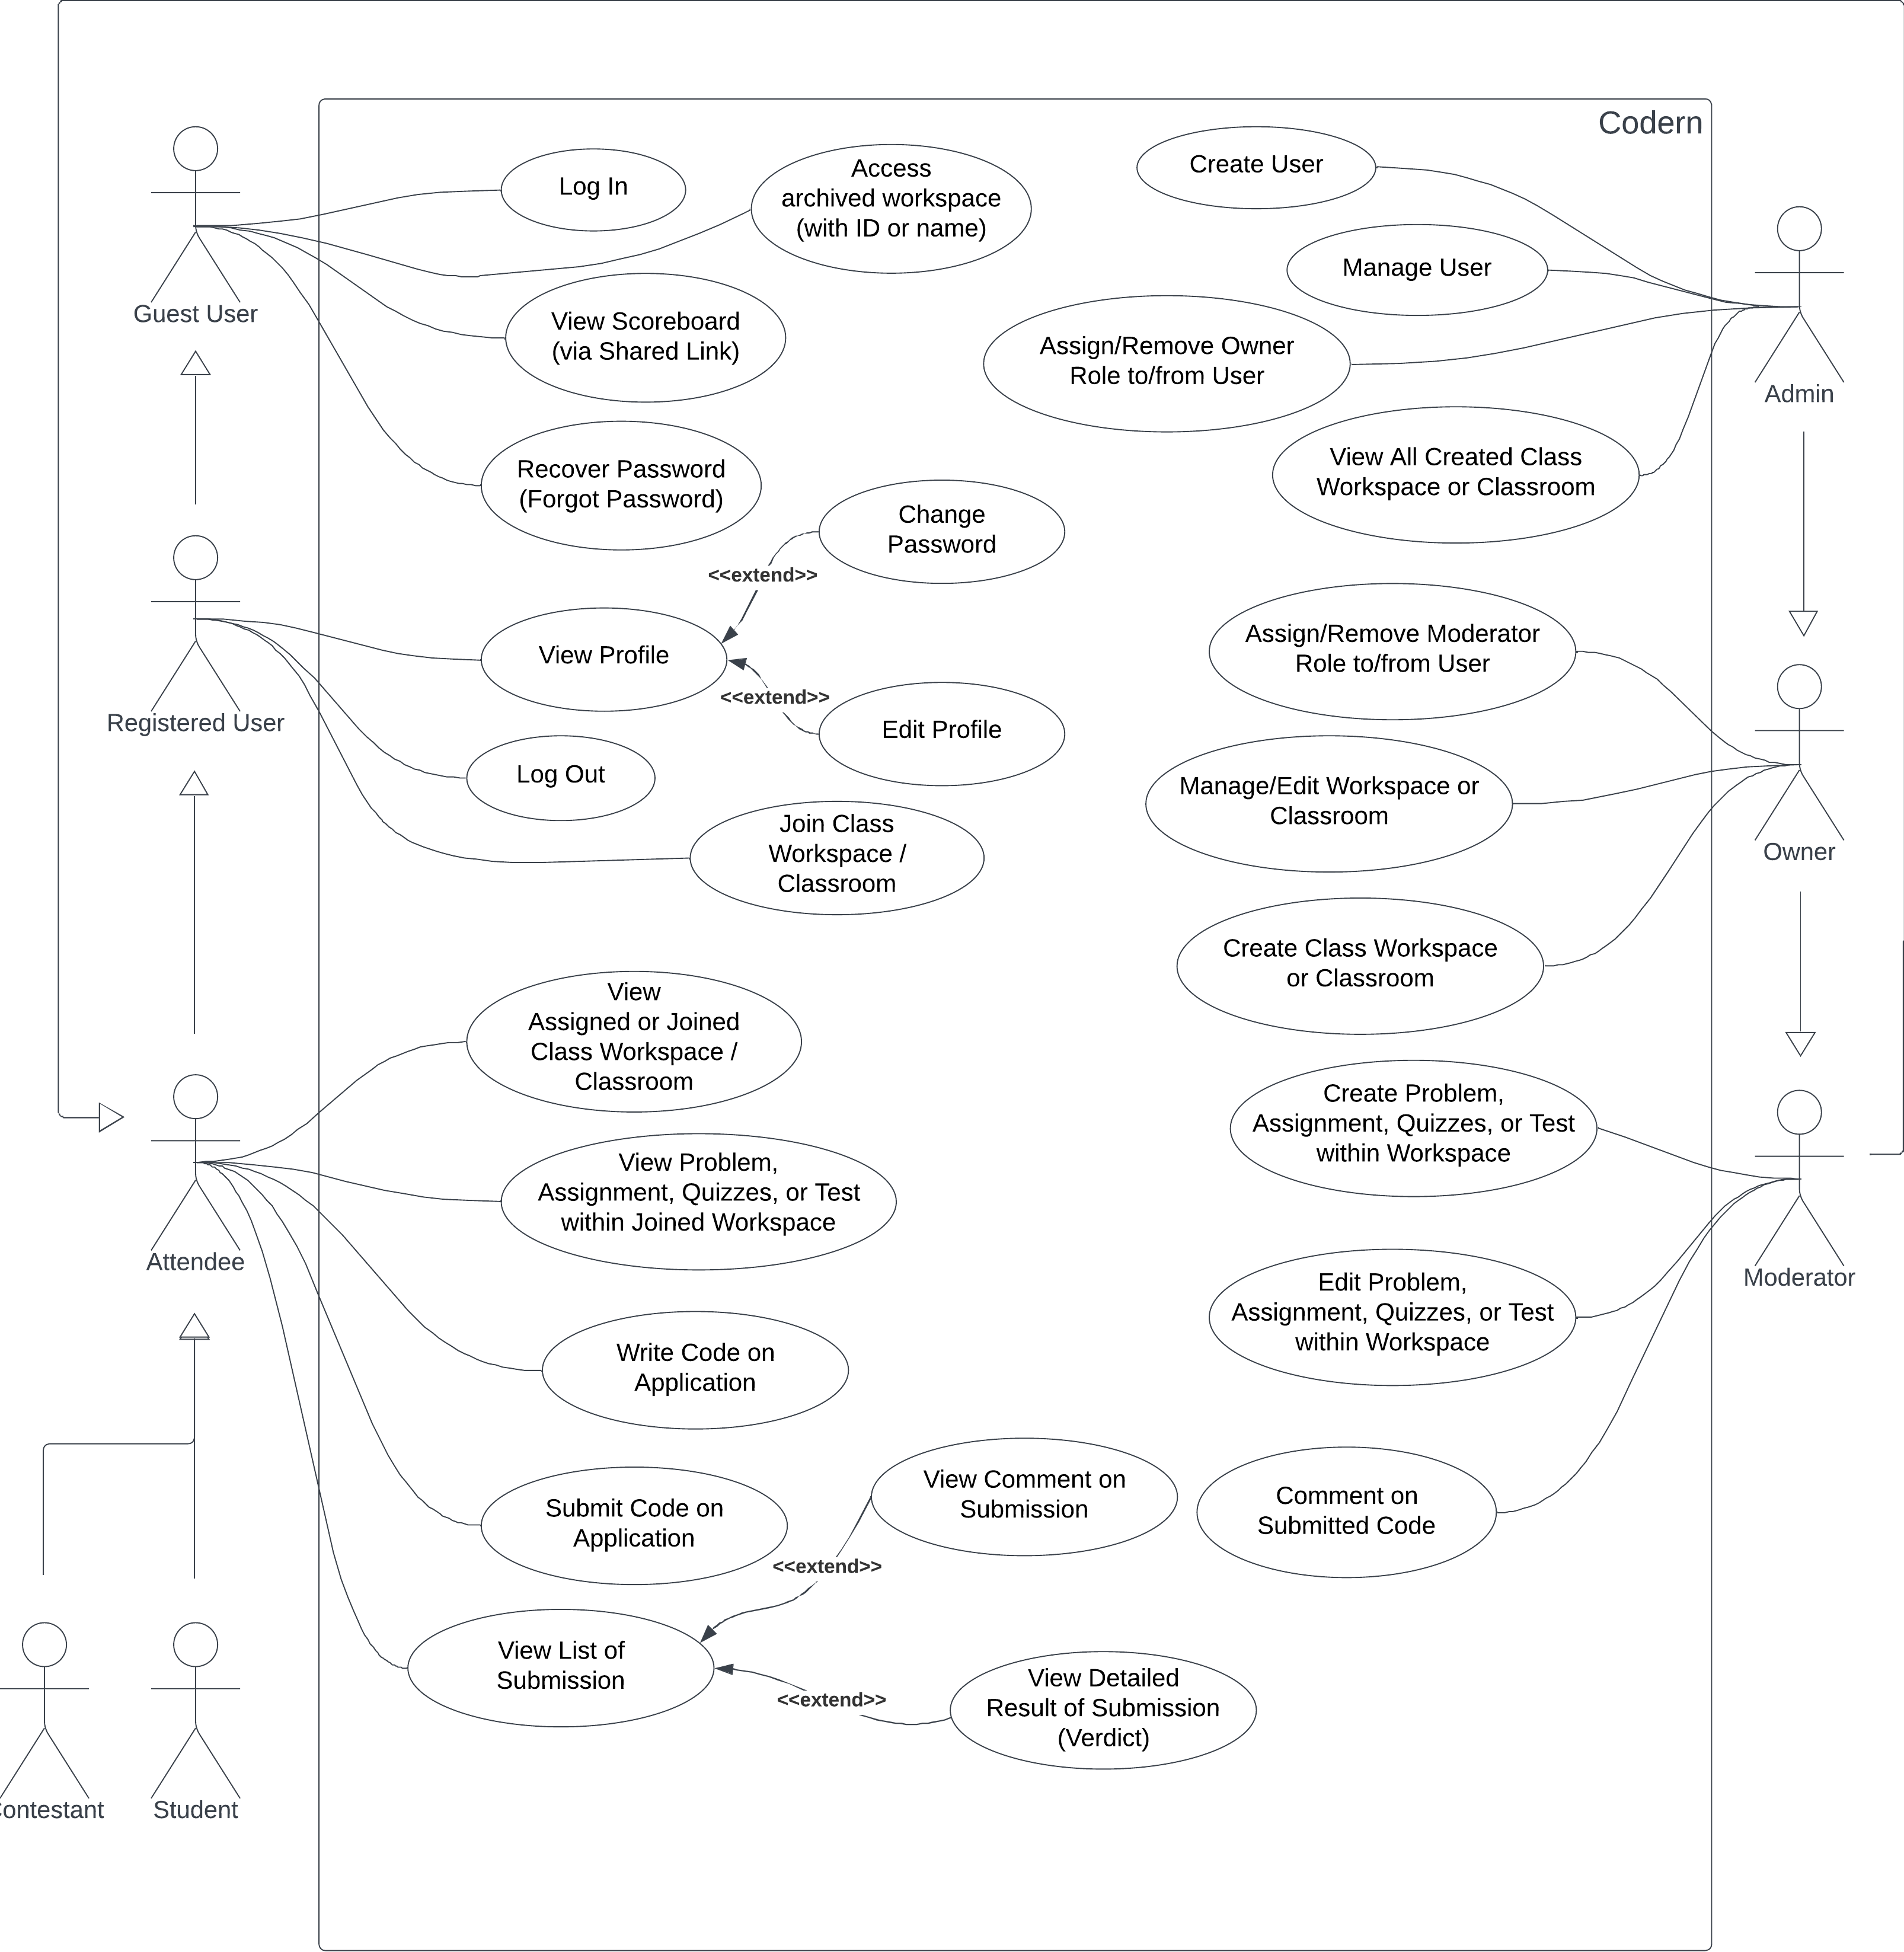
\includegraphics[width=15cm]{figure/diagram/usecase-v5.png}
        \caption[ภาพเเผนผังกรณีใช้งาน]{ภาพเเผนผังกรณีใช้งาน วาดด้วย \href{https://lucid.app/}{LucidChart}}
        \label{fig:usecase}
        \end{figure}
        \pagebreak
    \subsection{คำบรรยายแผนผังกรณีใช้งาน}
        \thaijustify{
            จาก\cref{fig:usecase} ในหัวข้อที่แล้ว เป็น... ในโครงงานซอฟต์แวร์นี้ได้แบ่งประเภทผู้ใช้ออกเป็น ?? ประเภท ได้แก่...
        }
        \subsubsection{Guest User (บุคคลทั่วไป)}
            \thaijustify{
                บุคคลทั่วไป สามารถเข้าใช้งาน feature พื้นฐานของซอฟต์แวร์ได้ดังนี้
            }
            \begin{enumerate}
                \item “Log In” คือ การล็อกอินเข้าสู่ระบบ
                \item “View Scoreboard (via Shared Link)” คือ การเข้าถึงตารางคะแนนด้วยลิงก์ที่ถูกแชร์มา
                \item “Recover Password” คือ การกู้คืนรหัสผ่าน กรณีที่หลงลืมหรือสูญหาย
            \end{enumerate}
        \subsubsection{Registered User (ผู้ใช้ทั่วไป)}
            \thaijustify{
                ผู้ใช้ทั่วไปก็คือบุคคลทั่วไปที่มีบัญชีในระบบ (Admin อาจได้สร้างไว้ให้ หรือไม่ก็สมัครเอง) โดยผู้ใช้ทั่วไปสามารถเข้าถึง feature พื้นฐานของซอฟต์แวร์ได้เหมือนกับบุคคลทั่วไป (Guest User) และยังสามารถเข้าใช้ feature เพิ่มเติมได้ดังต่อไปนี้...
            }
    \pagebreak
\section{สถาปัตยกรรมระบบ}
    \thaijustify{
        ...
    }
    \pagebreak
\section{ส่วนประสานต่อผู้ใช้}
    \thaijustify{
        สำหรับในส่วนหน้าประสานงานผู้ใช้หรือ User Interface (UI) ... ได้ออกแบบไว้ทั้งหมดดังนี้...
    }
    \begin{figure}[H]
    \centering
        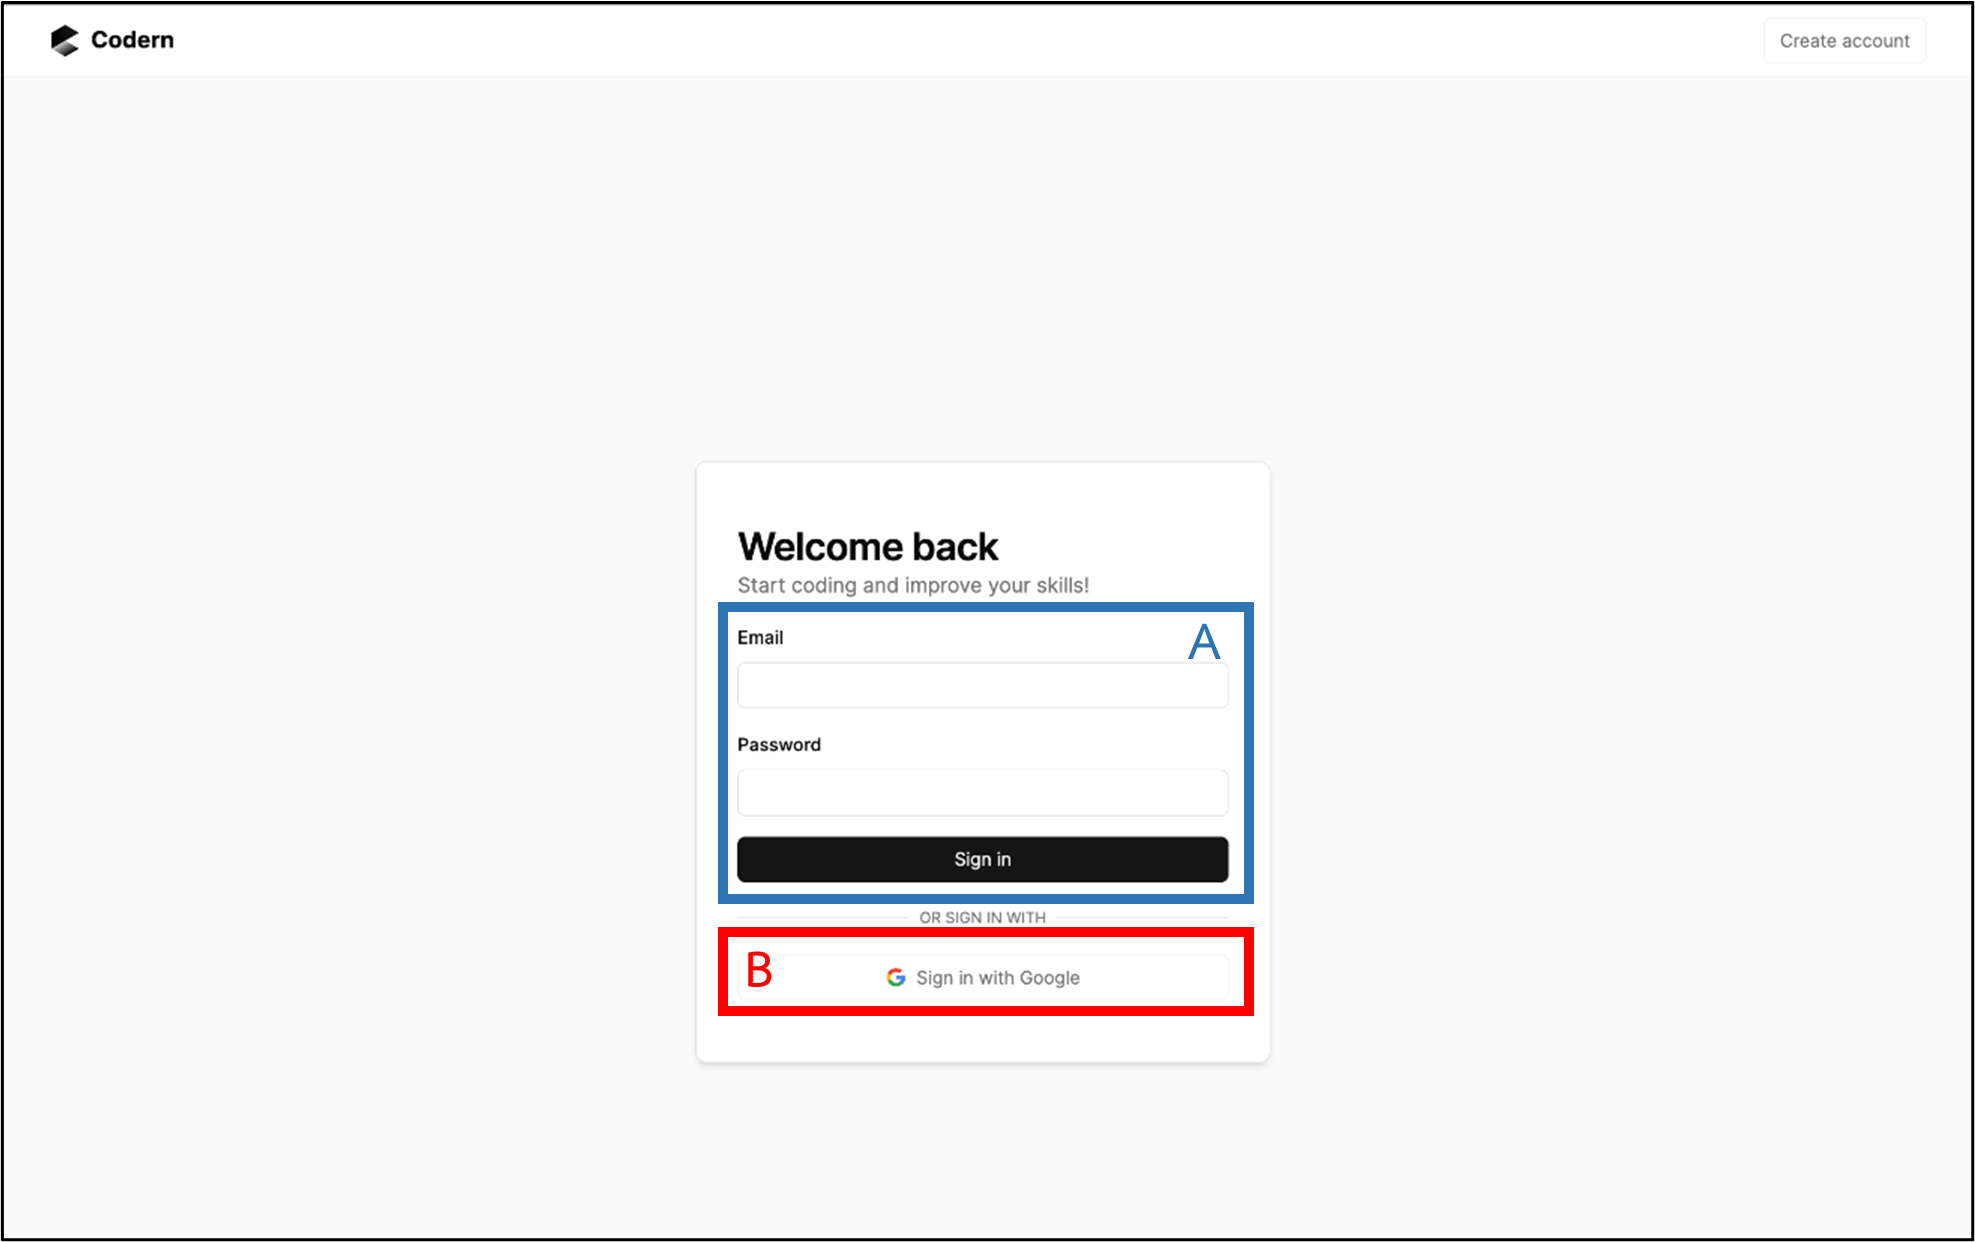
\includegraphics[width=15cm]{figure/ui/ui-login1.png}
        \caption[ส่วนประสานต่อผู้ใช้ หน้าเข้าสู่ระบบ]{ส่วนประสานต่อผู้ใช้ หน้าเข้าสู่ระบบ}
        \label{fig:ui-login}
    \end{figure}
    \thaijustify{
        ใน\cref{fig:ui-login} เป็นหน้าสำหรับล็อกอินเข้าระบบใช้งานทั้งหมดของซอฟต์แวร์ โดยสามารถเลือกล็อกอินได้สองวิธี; ด้วยอีเมลเเละรหัสผ่าน (กรอบสีน้ำเงิน A) และล็อกอินผ่านกูเกิ้ล (กรอบสีแดง B)...
    }  
\pagebreak
\section{โครงสร้างฐานข้อมูล}
    \thaijustify{
       ...
    }
    \pagebreak
    \subsection{คำบรรยายโครงสร้างฐานข้อมูล}
    \thaijustify{
        ในส่วนนี้ทางกลุ่มเราจะอธิบาย รายละเอียด... จากฐานข้อมูลในส่วนที่แล้ว...
    }
    \begin{enumerate}
        %% User's Relations
        \item \textbf{User}
            เป็นตารางที่เก็บข้อมูลของผู้ใช้แต่ละคน เช่นอีเมลล์, ชื่อ-นามสกุลขของผู้ใช้ เป็นต้น จากความสัมพันธ์ของตารางดังกล่าว กับตารางอื่น ๆ สามารถสรุปความสัมพันธ์ได้ดังนี้
            \begin{figure}[H]
                \centering
                \subfloat[แผนผังแสดงความสัมพันธ์ระหว่างตาราง User และ Session]{
                    \begin{tikzpicture}[auto,node distance=0.7cm]
                        % First Entity
                        \node[entity] (node1) {User};
                        % [grow=up,sibling distance=3cm]
                        % child {node[attribute] {Attribute 1}}
                        % child {node[attribute] {Attribute 2}}
                        % child[grow=left,level distance=3cm] {node[attribute] {Attribute 3}};
                        % Relationship
                        \node[relationship] (rel1) [right = of node1] {has};
                        % Second Entity
                        \node[entity] (node2) [right = of rel1]	{Session};
                        % Draw an edge between rel1 and node1; rel1 and node2
                        \path (rel1) edge node {\(1\)-\(1\)} 
                        (node1) edge node {\(1\)-\(m\)}	(node2);
                    \end{tikzpicture}
                    \label{fig:db-user-session}
                } \hspace{0.5cm}
                \subfloat[แผนผังแสดงความสัมพันธ์ระหว่างตาราง User และ Workspace]{
                    \begin{tikzpicture}[auto,node distance=0.7cm]
                        % First Entity
                        \node[entity] (node1) {User};
                        % Relationship
                        \node[relationship] (rel1) [right = of node1] {owns};
                        % Second Entity
                        \node[entity] (node2) [right = of rel1]	{Workspace};
                        % Draw an edge between rel1 and node1; rel1 and node2
                        \path (rel1) edge node {\(1\)-\(1\)} 
                        (node1) edge node {\(0\)-\(m\)}	(node2);
                    \end{tikzpicture}
                    \label{fig:db-user-workspace}
                } \\
                \subfloat[แผนผังแสดงความสัมพันธ์ระหว่างตาราง User และ WorkspaceParticipant]{
                    \begin{tikzpicture}[auto,node distance=0.7cm,]
                        % First Entity
                        \node[entity] (node1) {User};
                        % Relationship
                        \node[relationship] (rel1) [right = of node1] {becomes};
                        % Second Entity
                        \node[entity] (node2) [right = of rel1]	{WorkspaceParticipant};
                        % Draw an edge between rel1 and node1; rel1 and node2
                        \path (rel1) edge node {\(1\)-\(1\)} 
                        (node1) edge node {\(0\)-\(m\)}	(node2);
                    \end{tikzpicture}
                    \label{fig:db-user-workspace_participant}
                } \\
                \subfloat[แผนผังแสดงความสัมพันธ์ระหว่างตาราง User และ Submission]{
                    \begin{tikzpicture}[auto,node distance=0.7cm]
                        % First Entity
                        \node[entity] (node1) {User};
                        % Relationship
                        \node[relationship] (rel1) [right = of node1] {submit};
                        % Second Entity
                        \node[entity] (node2) [right = of rel1]	{Submission};
                        % Draw an edge between rel1 and node1; rel1 and node2
                        \path (rel1) edge node {\(1\)-\(1\)} 
                        (node1) edge node {\(0\)-\(m\)}	(node2);
                    \end{tikzpicture}
                    \label{fig:db-user-submission}
                }
                \caption[กลุ่มแผนผังแสดงความสัมพันธ์ของตาราง User]{กลุ่มแผนผังแสดงความสัมพันธ์ของตาราง User}
                \label{fig:db-user}
            \end{figure}
            \begin{itemize}
                \item จากรูปที่~\ref{fig:db-user-session} ผู้ใช้สามารถที่จะเข้าสู่ระบบได้หลายเครื่องพร้อม ๆ กัน ก็คือผู้ใช้เข้าสู่ระบบได้ (has) หลาย Session พร้อมกัน
                \item จากรูปที่~\ref{fig:db-user-workspace} ผู้ใช้สามารถที่จะครอบครอง (owns) Workspace ได้มากกว่า 1 Workspace
                \item จากความสัมพันธ์ในรูป~\ref{fig:db-user-workspace_participant} ผู้ใช้สามารถที่จะเป็นคนเข้าร่วม (join workspace) ในกลุ่มเรียนหรือห้องเรียน (หรือ Workspace Participant) ได้มากกว่า 1 ห้องเรียนหรือกลุ่มเรียน หรือ Workspace
                \item จากรูปที่~\ref{fig:db-user-submission} ผู้ใช้สามารถที่จะส่ง (submit) ได้มากกว่า 1 ห้องเรียนหรือกลุ่มเรียน หรือ Workspace
            \end{itemize}
        %% Session's Relations
        \item \textbf{Session}
            เป็นตารางที่จะเก็บข้อมูล Session หรือข้อมูลเครื่อง ข้อมูลช่องทางที่ผู้ใช้เข้าสู่ระบบ สามารถสรุปความสัมพันธ์ได้ดังนี้
            \begin{itemize}
                \item ถึงเเม้ผู้ใช้หนึ่งท่านสามารถที่จะมีได้หลาย Session คือผู้ใช้สามารถเข้าสู่ระบบได้หลายเครื่องพร้อมก่อน แต่ Session เป็นของผู้ใช้แค่คนเดียวเท่านั้นตามรูปที่~\ref{fig:db-user-session}
            \end{itemize}
        %% Workspace's Relations
        \item \textbf{Workspace}
            เป็นตารางที่สร้างขึ้นมาเก็บข้อมูลห้องเรียนหรือกลุ่มเรียน (Workspace) มีความสัมพันธ์กับตารางอื่นดังต่อไปนี้...
   \end{enumerate} 
    \subsection{พจนานุกรมข้อมูล}
        \thaijustify{
            ในส่วนนี้ จะเป็นพจนานุกรม... ที่อยู่ในแผนภาพฐานข้อมูลในหัวข้อก่อน   
        }
        \begin{table}[H]
            \centering
            \caption{พจนานุกรมข้อมูลของตาราง User}\label{tbl:data-dict-user}
            \begin{tabular}{p{2cm}|p{4cm}p{2cm}p{3cm}p{2cm}} \hline\hline
                Attribute Name & Description & Data Type & Constraints & References \\ \hline\hline
                id & รหัส ID การส่งงาน & bigint & Primary Key & - \\
                a\_id & ID ของโจทย์ & bigint & Foreign Key, Not Null & Assign \\
                uid & ID ของผู้ใช้ & varchar(64) & Foreign Key, Not Null & User \\
                ... & ... & varchar(128) & Not Null & - \\
                ... & ... & longtext & - & - \\ \hline\hline
            \end{tabular}   
        \end{table}
    \pagebreak
\section{แผนผัง UML}
    \thaijustify{
        สำหรับในส่วนนี้ จะแสดงและบรรยาย... เเผนผัง UML ที่ได้วาดมา...
    }
\pagebreak

%%%%%%%%%%%%%%%%%%%%% Results and Discussions %%%%%%%%%%%%%%%%%%%%%%%%

\chapter{ผลการดำเนินงาน}
\thaijustify{
    ในบทที่ 4 จะกล่าวบรรยายและอภิปรายผล... ของโครงการ...
}
\thaijustify{
    ในปีการศึกษาที่ผ่านมา... ตามในแผน... ทางกลุ่มได้ทำ
}
\section{ผลจากการดำเนินการ}

\pagebreak
\section{ผลลัพธ์จากการทดลองเปิดใช้งานซอฟต์แวร์}
   
\pagebreak
\section{การอภิปรายผลจากการดำเนินการ}

\pagebreak

%%%%%%%%%%%%%%%%%%%%%%%%%%% Conclusions %%%%%%%%%%%%%%%%%%%%%%%%%%%%%

\chapter{บทสรุป}
    ในบทที่ 5 คณะผู้จัดทำจะกล่าวสรุป... พร้อมอธิบายปัญหาที่พบเจอ พร้อมอธิบายวิธีการแก้... แล้วให้คำแนะนำกับข้อเสนอแนะ...
\section{สรุปผลโครงงาน}

\pagebreak
\section{ปัญหาที่พบและการแก้ไข}

\pagebreak
\section{ข้อเสนอแนะสำหรับการพัฒนาต่อในอนาคต}

%%%%%%%%%%%%%%%%%%%%%%%%%%% Bibliography %%%%%%%%%%%%%%%%%%%%%%%%%%%%
%: Comment this in your report to show only references you have
%: cited. Otherwise, all the references below will be shown.
% \nocite{*}

% Use the kmutt.bst for bibtex bibliography style 
% You must have cpe.bib and string.bib in the correct directory
% You may go to file .bbl to manually edit the bib items.

%: Sept, 2021 by Thanin
%: Improve url breaks to prevent unnecessary big white spaces in some cases
\makeatletter
\g@addto@macro{\UrlBreaks}{\UrlOrds}
\makeatother

%: July, 2024 by Jatetanan
%: Add biblatex for managing bibs
%: Uncomment this if you're using biblatex
% \printbibliography[heading=bibintoc,title={บรรณานุกรม}]

%: Uncomment \bibliographystyle and \bibliography if you're not using biblatex
%: References style
%: Examples: \bibliographystyle{bibstyle/kmutt} 
\bibliographystyle{bib/ieee}

%: References files
%: Examples: \bibliography{example/string,example/string2,example/cpe}
\bibliography{bib/codern}

%%%%%%%%%%%%%%%%%%%%%%%%%%% Appendices %%%%%%%%%%%%%%%%%%%%%%%%%%%%%%
\appendix{แผนผังและแบบแปลนโครงสร้างซอฟต์แวร์ปรับใหม่}

    \begin{figure}[H]
        \centering
            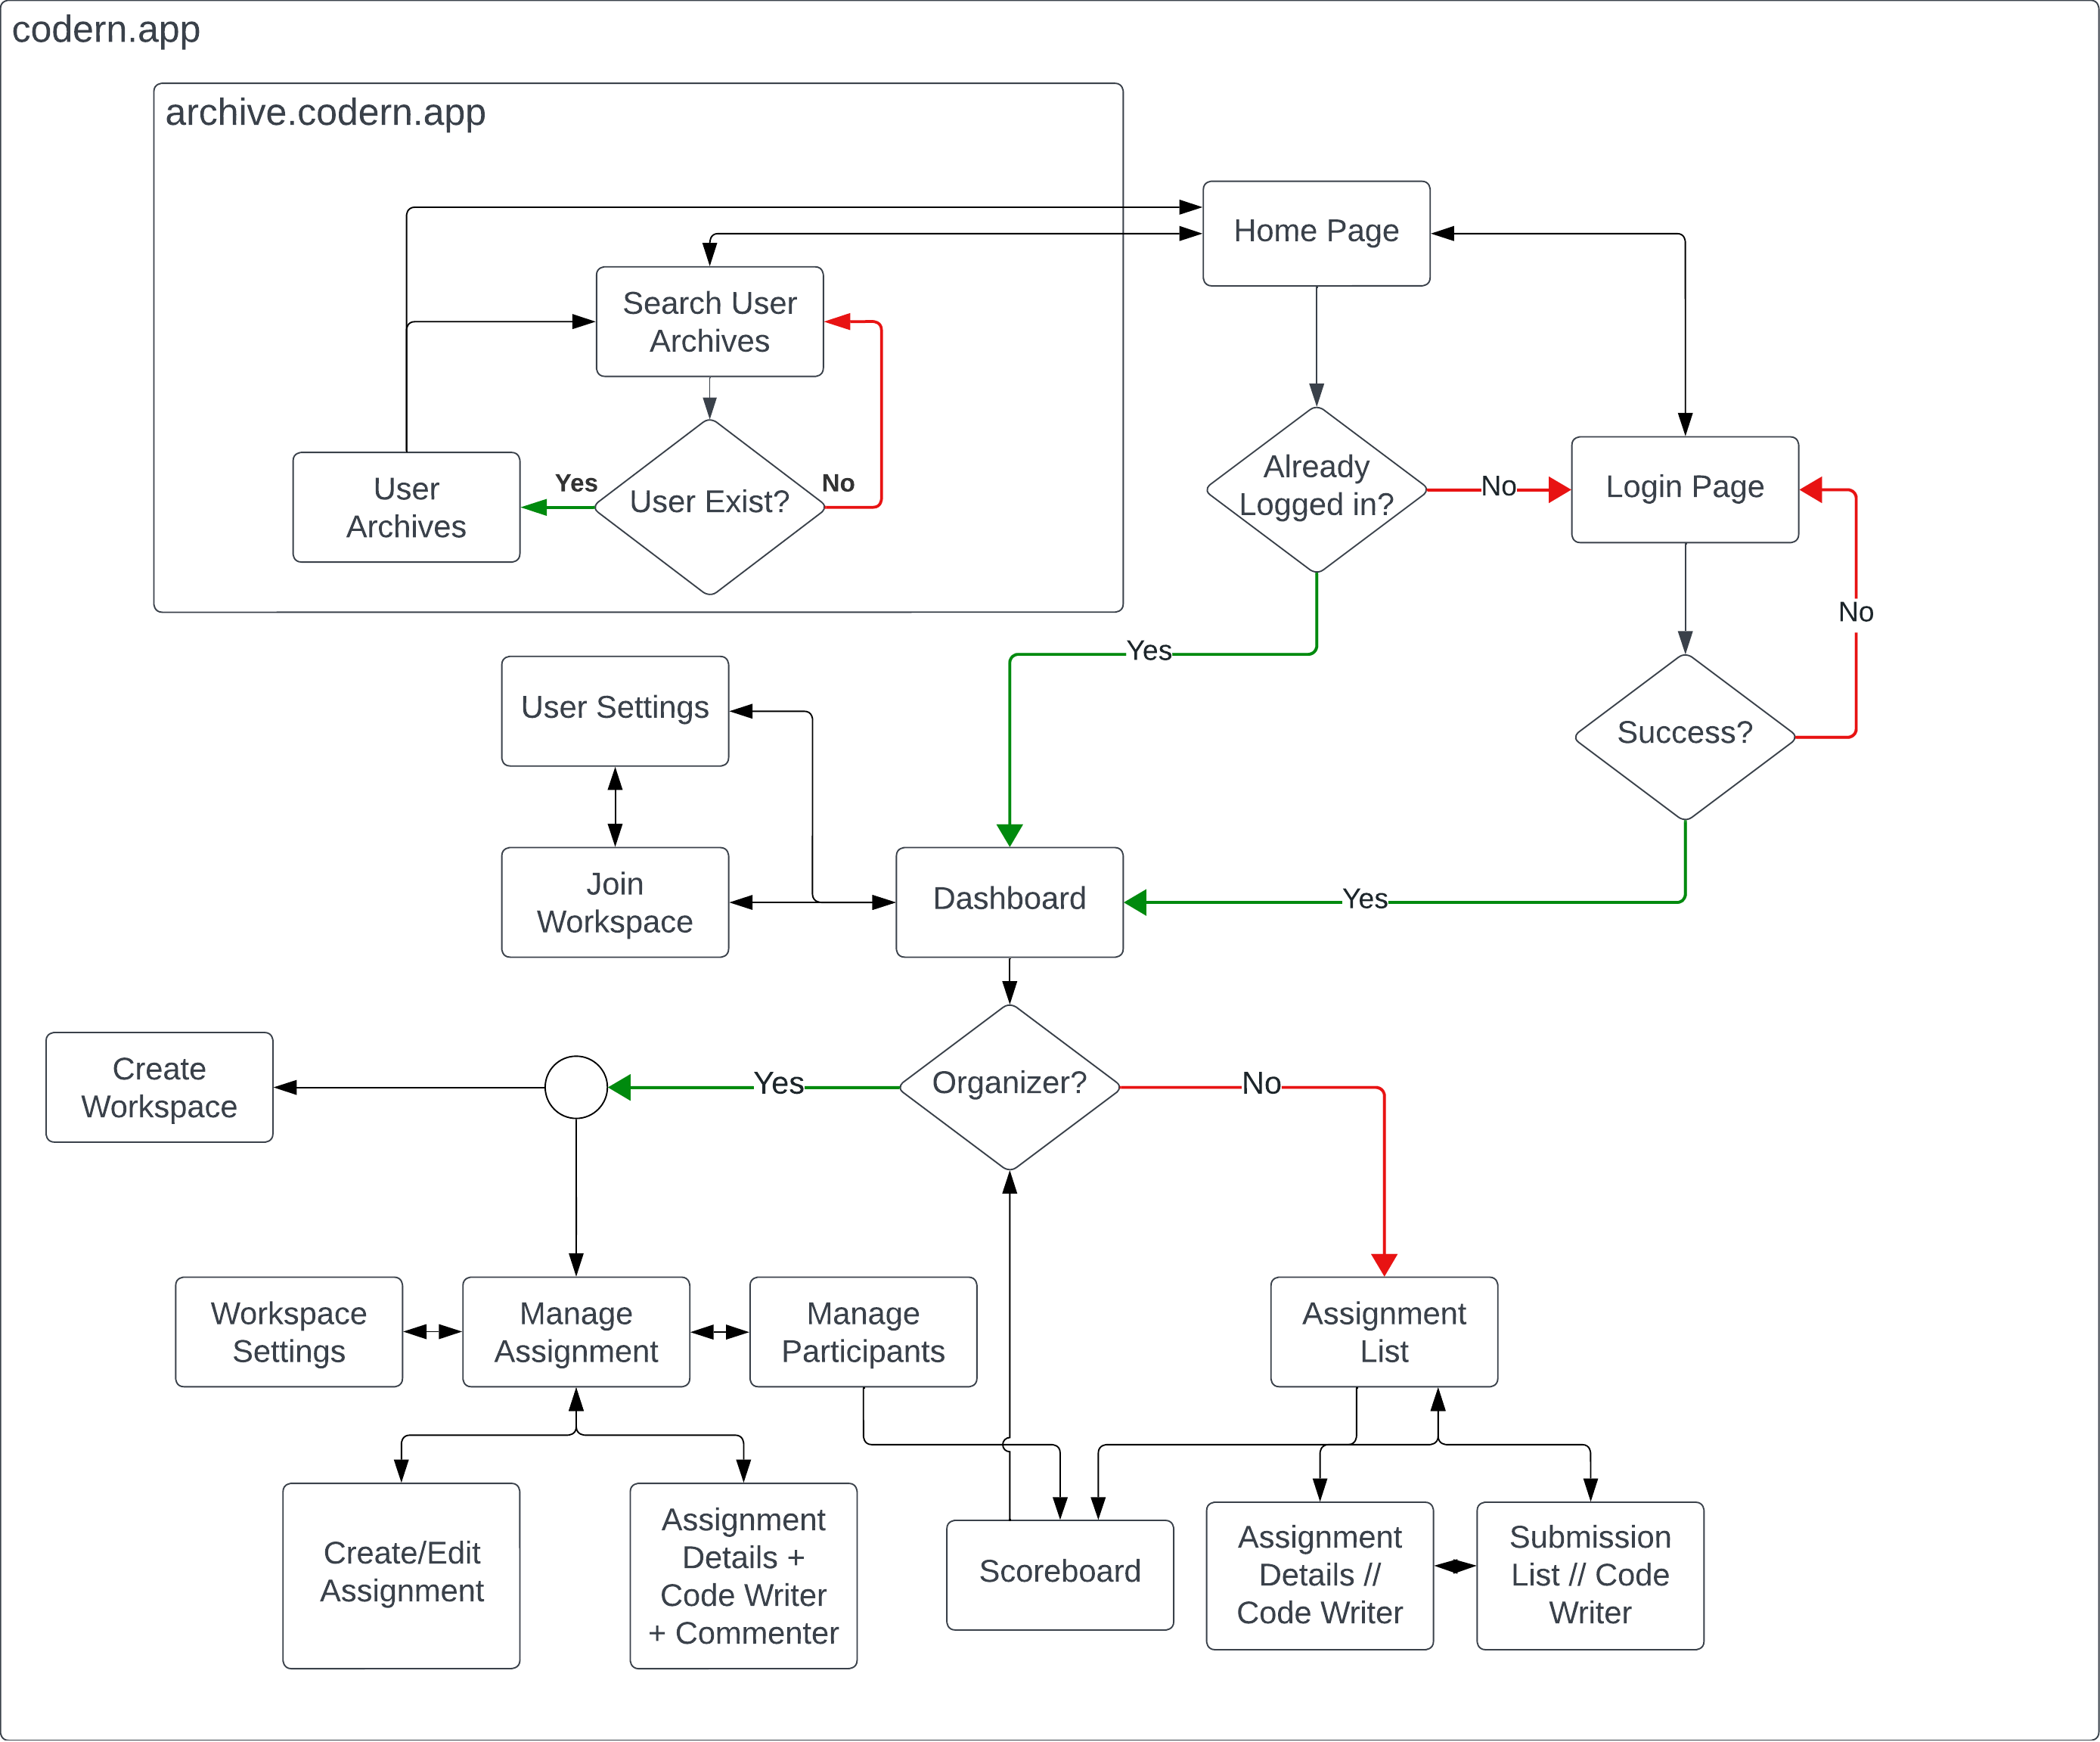
\includegraphics[width=15cm]{figure/diagram/navigation-v3.png}
        \label{fig:appendix-nav-map}
        \caption[แผนผังการสัญจรและนำทางหน้าเว็บไซต์ที่มีแบบใหม่]{แผนผังการสัญจรและนำทางหน้าเว็บไซต์ที่มีแบบใหม่}
    \end{figure}
    
    \centering\noindent{\large\bf แผนผังการสัญจรหน้าเว็บไซต์ที่มีการเปลี่ยนแปลงไปจากเดิม แบบใหม่มีการแยก View ของ Organizer กับ User ธรรมดาอย่างชัดเจน ไม่มีการ Switch ไปมาอีกต่อไป} \\

\appendix{ตัวอย่างซอร์สโค้ดของซอฟต์แวร์โครงการ}

%%%%%% Dependency Injection %%%%%%
\noindent{\large\bf ตัวอย่างการทำ Dependency Injection ระหว่างไฟล์ User's Usecase กับไฟล์ User's Repository} \\

    \begin{lstlisting}[label={lst:appendix-user-domain}, caption={ชุดคำสั่งที่นิยาม Interface ของ User Repository และ User Usecase}]
    // ...
    type UserRepository interface {
        Create(user *User) error
        Get(id string) (*User, error)
        GetBySessionId(id string) (*User, error)
        GetByEmail(email string, provider AuthProvider) (*User, error)
        Update(user *User) error
    }
    
    type UserUsecase interface {
        Create(email string, password string) (*User, error)
        CreateFromGoogle(id string, email string, name string) (*User, error)
        Get(id string) (*User, error)
        GetBySessionId(id string) (*User, error)
        GetByEmail(email string, provider AuthProvider) (*User, error)
        Update(id string, user *UpdateUser) error
        UpdatePassword(id string, oldPlainPassword string, newPlainPassword string) error
    }
    // ...
    \end{lstlisting}
    
    \begin{lstlisting}[label={lst:appendix-user-usecase}, caption={ชุดคำสั่งสร้างและนิยาม UserUsecase ที่มีการ Implement UserRepository}]
    // ...
    type userUsecase struct {
        seaweedfs      *platform.SeaweedFs
        userRepository domain.UserRepository
        sessionUsecase domain.SessionUsecase
    }
    
    func NewUserUsecase(
        seaweedfs *platform.SeaweedFs,
        userRepository domain.UserRepository,
        sessionUsecase domain.SessionUsecase,
    ) domain.UserUsecase {
        return &userUsecase{
            seaweedfs:      seaweedfs,
            userRepository: userRepository,
            sessionUsecase: sessionUsecase,
        }
    }
    // ...
    \end{lstlisting}
    
\pagebreak
\appendix{รายงานผลการทำงานของซอฟต์แวร์}
\noindent{\large\bf สรุปผลการทำงานของซอฟต์แวร์ ในช่วงกิจกรรมการแข่งขันเขียนโปรแกรมภาษาคอมพิวเตอร์ทั้ง 3 รอบ ที่จัดที่ภาควิชาวิศวกรรมคอมพิวเตอร์ คณะวิศวกรรมศาสตร์ มหาลัยเทคโนโลยีพระจอมเกล้าธนบุรี} \\

\begin{figure}[H]
    \centering
    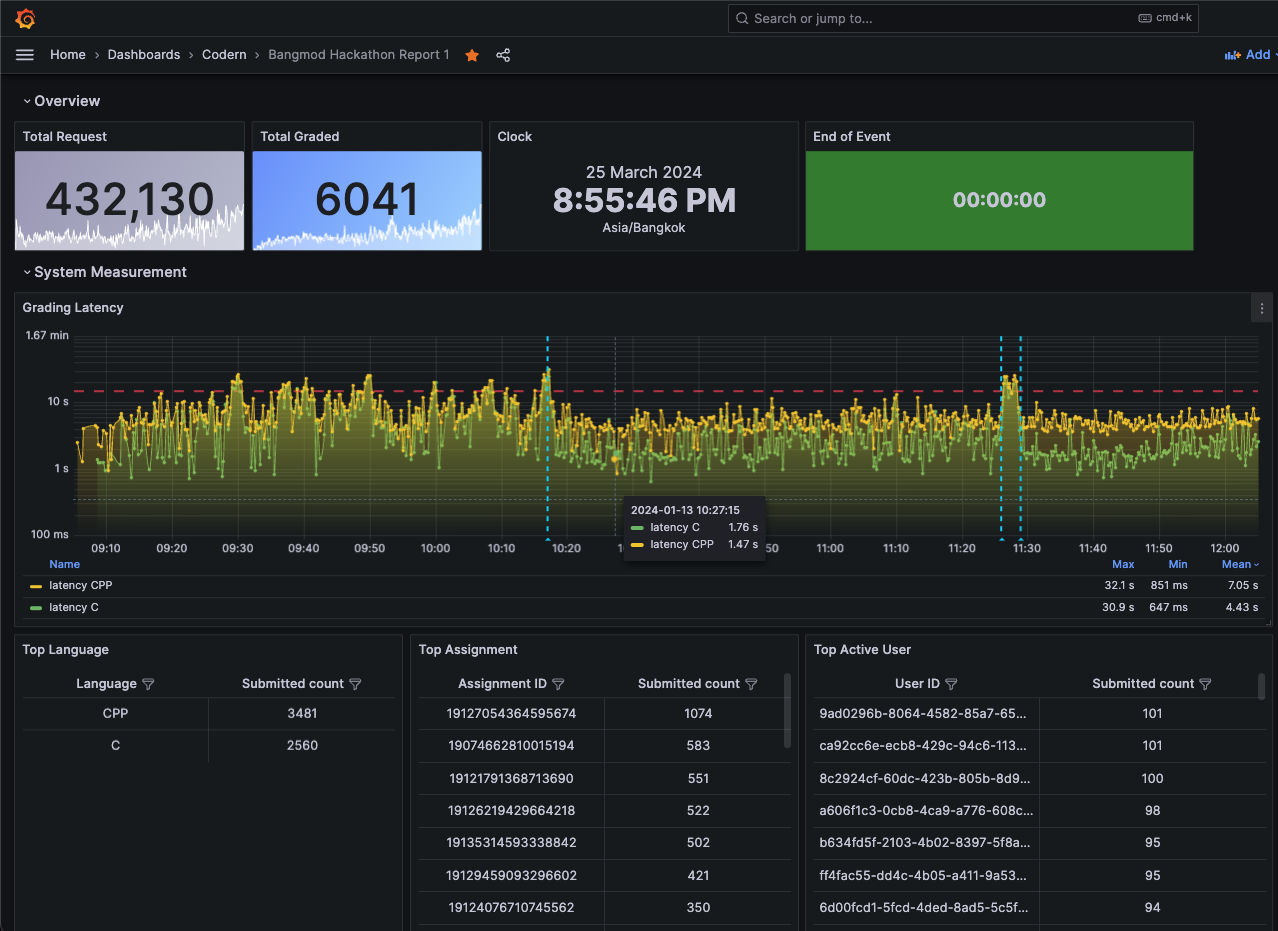
\includegraphics[width=12cm]{figure/results/grafana/grafana-bmh1-report.png}
    \caption[หน้ารายงานผลการใช้งานซอฟต์แวร์ ของการแข่งขันเขียนโปรแกรมภาษาคอมพิวเตอร์รอบที่ 1 ฉบับรายงาน]{หน้ารายงานผลการใช้งานซอฟต์แวร์ ของการแข่งขันเขียนโปรแกรมภาษาคอมพิวเตอร์รอบที่ 1 ฉบับรายงาน (Report version)}
    \label{fig:res-grafana-bmh1-report}
\end{figure}

\begin{figure}[H]
    \centering
    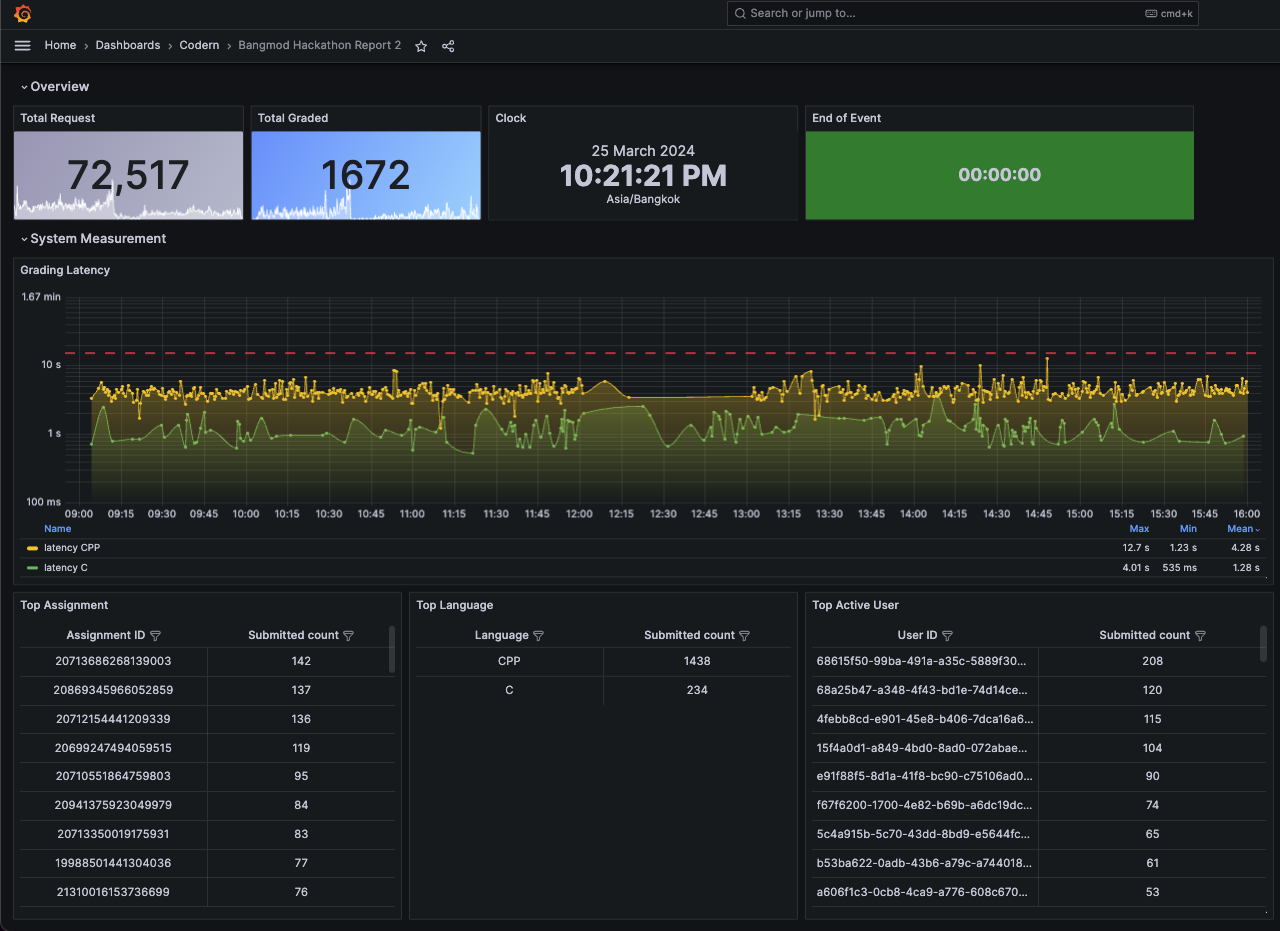
\includegraphics[width=12cm]{figure/results/grafana/grafana-bmh2-report.png}
    \caption[หน้ารายงานผลการใช้งานซอฟต์แวร์ ของการแข่งขันเขียนโปรแกรมภาษาคอมพิวเตอร์รอบที่ 2-3 ฉบับรายงาน]{หน้ารายงานผลการใช้งานซอฟต์แวร์ ของการแข่งขันเขียนโปรแกรมภาษาคอมพิวเตอร์รอบที่ 2-3 ฉบับรายงาน (Report version)}
    \label{fig:res-grafana-bmh2-report}
\end{figure}

\pagebreak

\appendix{ผลลัพธ์จากแบบสำรวจความพึงพอใจการใช้งานซอฟต์แวร์ (เพิ่มเติม)}

\begin{figure}[H]
    \centering
    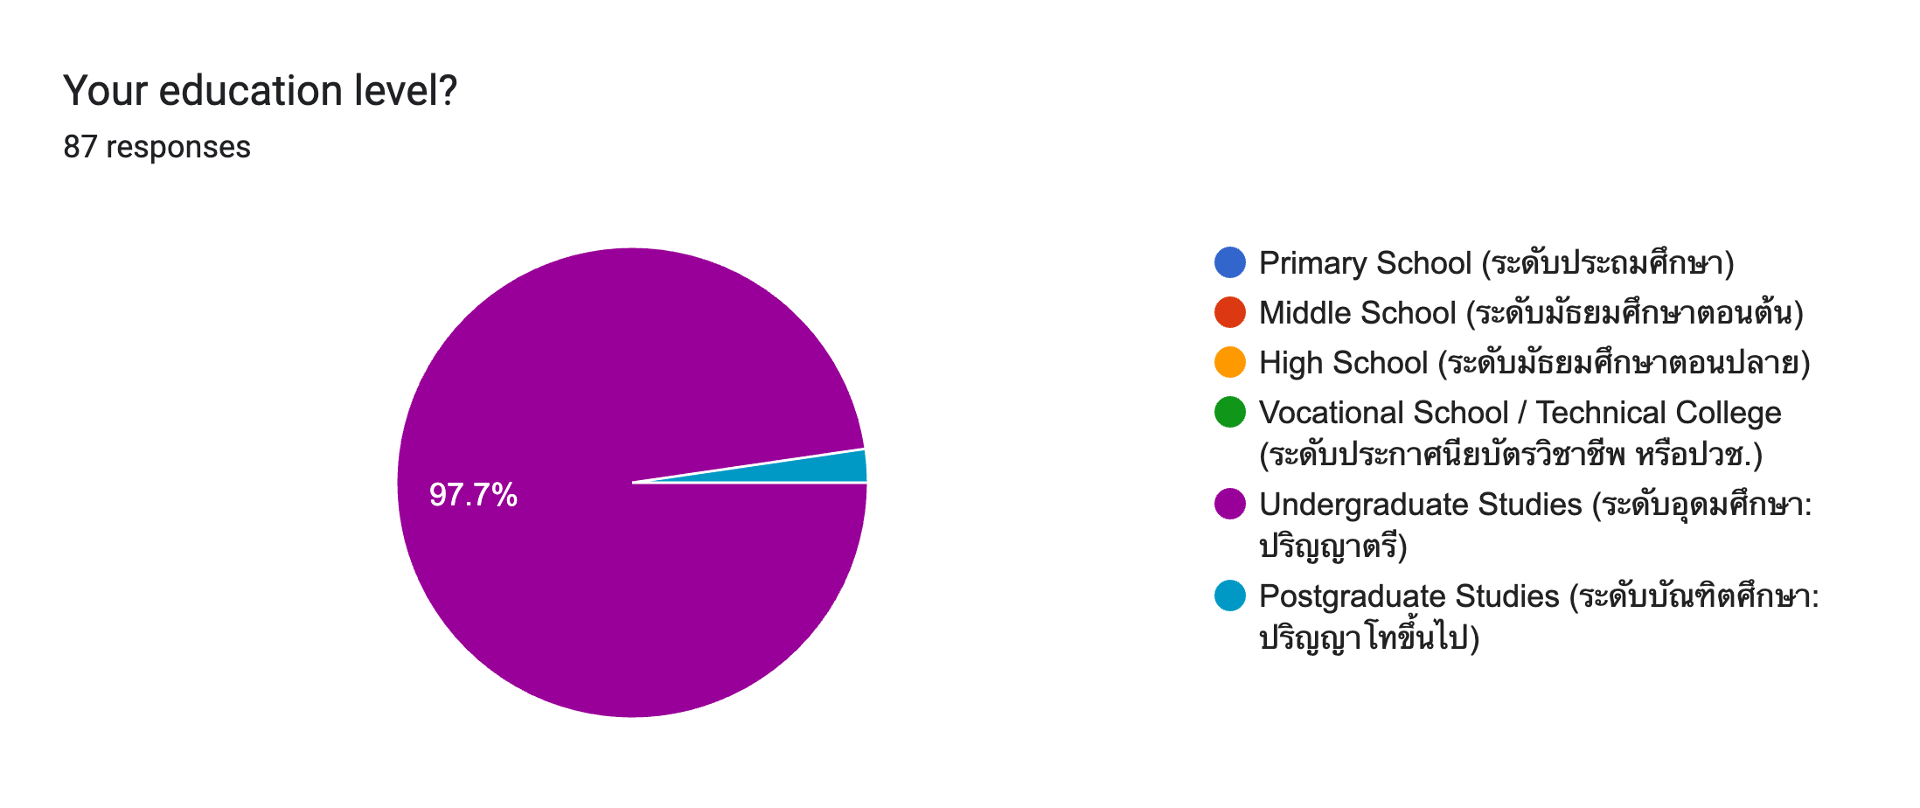
\includegraphics[width=15cm]{figure/results/survey/survey-education-lvl.png}
    \caption[ผลสำรวจแบบฟอร์มสำรวจความพึงพอใจผู้ใช้ต่อระบบซอฟต์แวร์ (ระดับการศึกษา)]{ผลสำรวจแบบฟอร์มสำรวจความพึงพอใจผู้ใช้ต่อระบบซอฟต์แวร์ เรื่องระดับการศึกษาของผู้ตอบแบบสอบถาม}
\end{figure}

\begin{figure}[H]
    \centering
    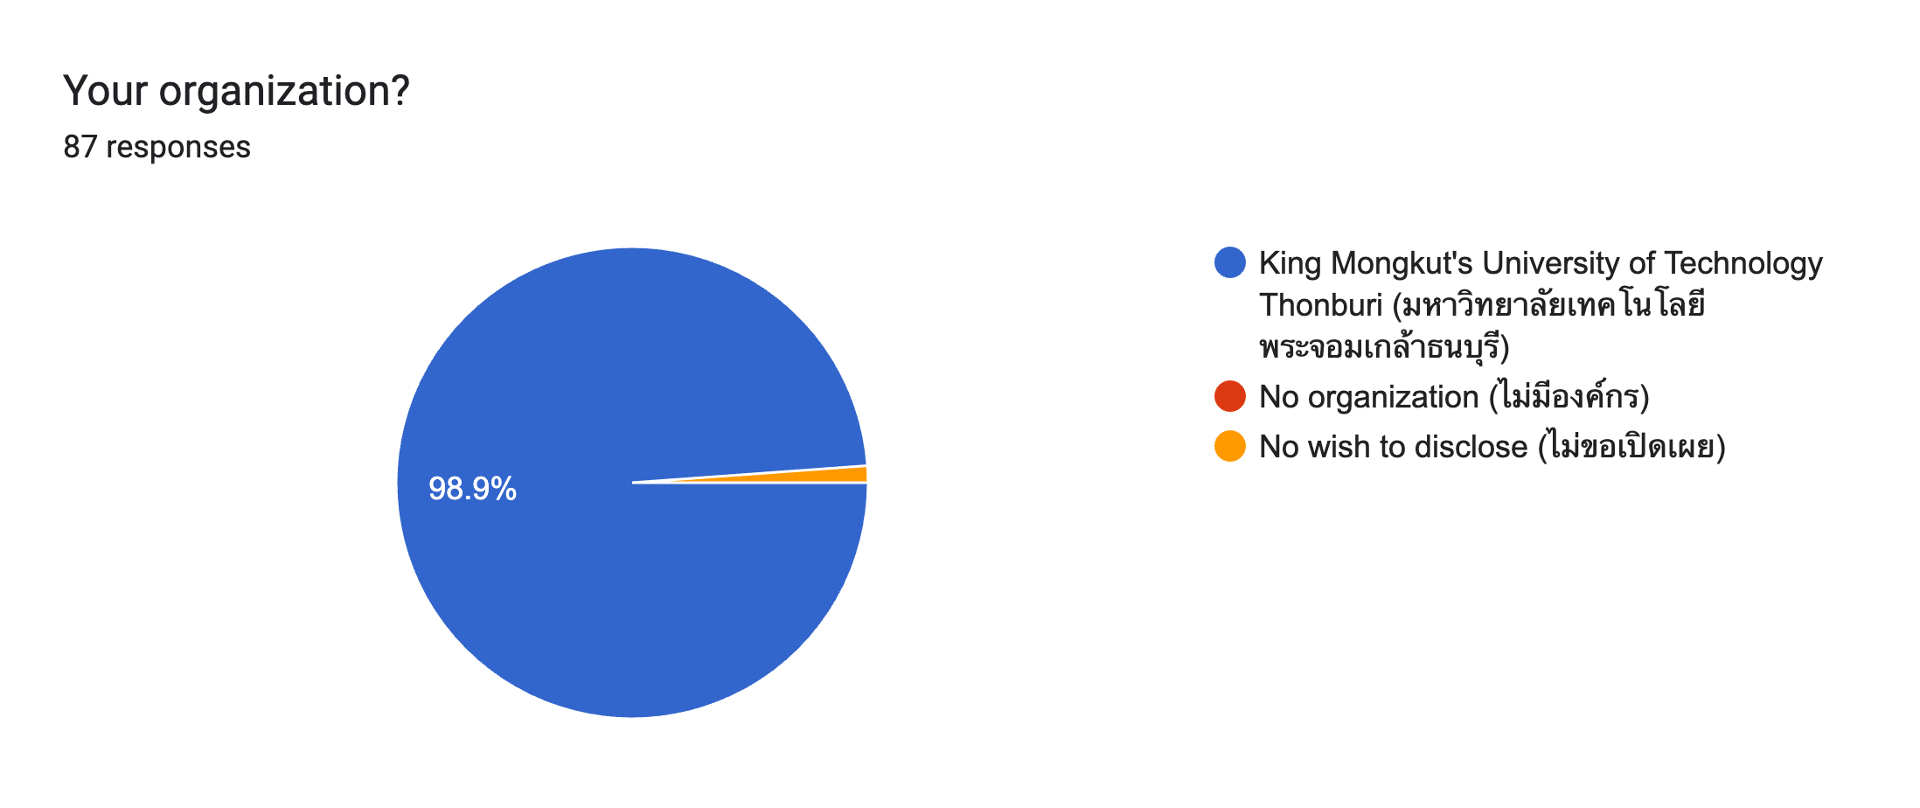
\includegraphics[width=15cm]{figure/results/survey/survey-org.png}
    \caption[ผลสำรวจแบบฟอร์มสำรวจความพึงพอใจผู้ใช้ต่อระบบซอฟต์แวร์ (องค์กร)]{ผลสำรวจแบบฟอร์มสำรวจความพึงพอใจผู้ใช้ต่อระบบซอฟต์แวร์ เรื่ององค์กรของผู้ตอบแบบสอบถาม}
\end{figure}

\begin{figure}[H]
    \centering
    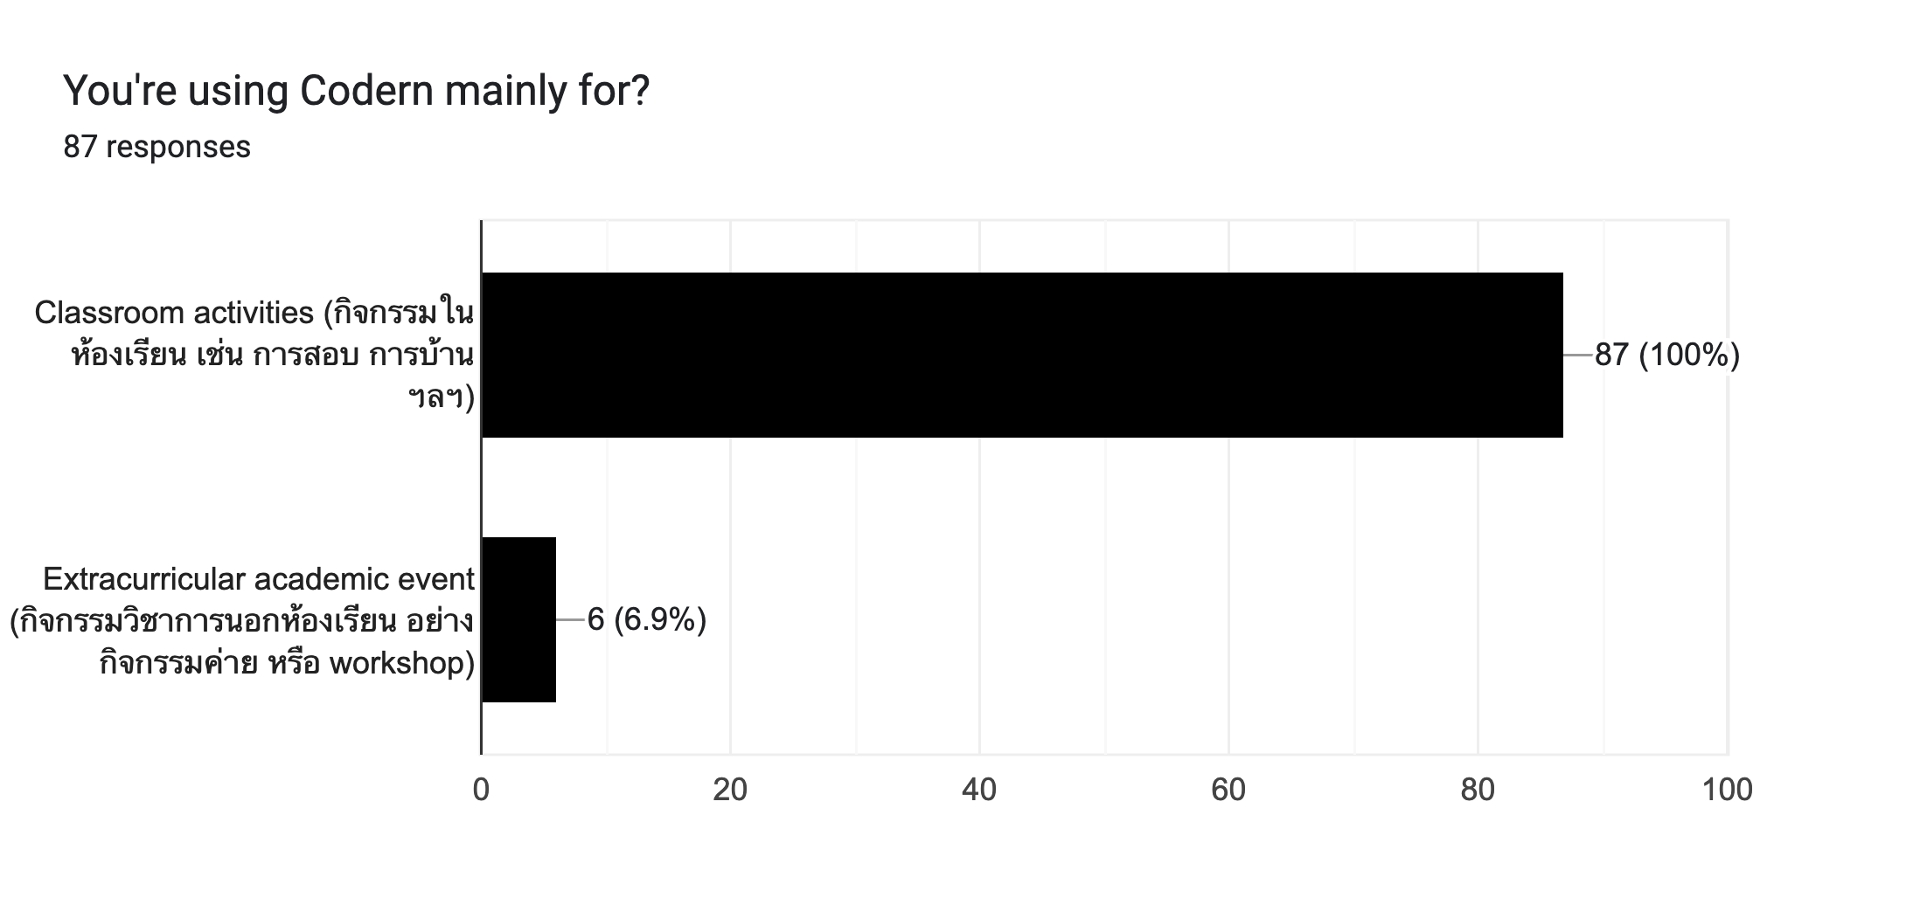
\includegraphics[width=15cm]{figure/results/survey/survey-usage-purpose.png}
    \caption[ผลสำรวจแบบฟอร์มสำรวจความพึงพอใจผู้ใช้ต่อระบบซอฟต์แวร์ (จุดมุ่งหมายของการใช้งานซอฟต์แวร์)]{ผลสำรวจแบบฟอร์มสำรวจความพึงพอใจผู้ใช้ต่อระบบซอฟต์แวร์ เรื่องจุดมุ่งหมายของการใช้งานซอฟต์แวร์}
\end{figure}

\begin{figure}[H]
    \centering
    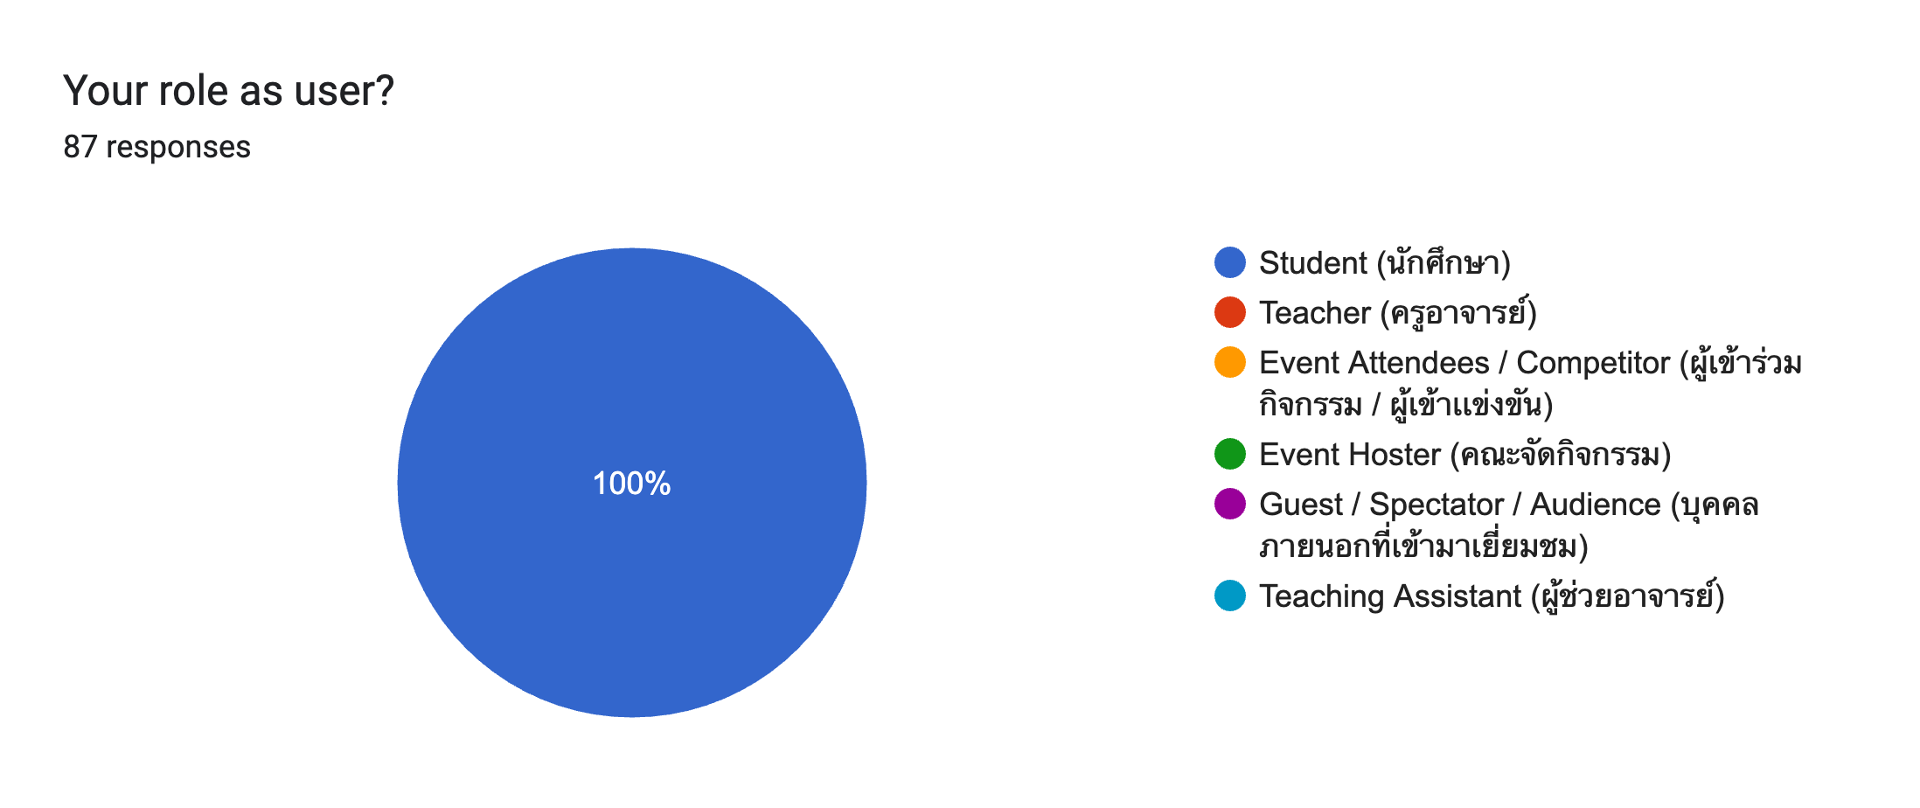
\includegraphics[width=15cm]{figure/results/survey/survey-user-role.png}
    \caption[ผลสำรวจแบบฟอร์มสำรวจความพึงพอใจผู้ใช้ต่อระบบซอฟต์แวร์ (บทบาทการใช้งาน)]{ผลสำรวจแบบฟอร์มสำรวจความพึงพอใจผู้ใช้ต่อระบบซอฟต์แวร์ เรื่องบทบาทการใช้งานของผู้ตอบแบบสอบถาม}
\end{figure}

\end{document}

%%%%%%%%%%%%%%%%%%%%%%%%%% REPORT END %%%%%%%%%%%%%%%%%%%%%%%%%%%%%%%
